\documentclass[english, aip, jcp, priprint, graphicx,floatfix]{revtex4-1}
\usepackage{amsmath}
\usepackage{amsthm}
\usepackage{amssymb}
\usepackage{mathrsfs}
\usepackage{bbm,latexsym}
\usepackage{graphicx}
\usepackage{cancel}
\usepackage{enumitem}

%%%%%%%%%% Start TeXmacs macros
\newcommand{\mathd}{\mathrm{d}}
\newcommand{\nin}{\not\in}
\newcommand{\tmop}[1]{\ensuremath{\operatorname{#1}}}
\newcommand{\tmtextbf}[1]{{\bfseries{#1}}}
\newtheorem{definition}{Definition}
\newtheorem{proposition}{Proposition}
\newtheorem{theorem}{Theorem}
\newtheorem{lemma}{Lemma}
\newtheorem{algorithm}{Algorithm}
%%%%%%%%%% End TeXmacs macros

\draft % marks overfull lines with a black rule on the right

\theoremstyle{plain}
\newtheorem{thm}{\protect\theoremname}
\newtheorem*{thm*}{\protect\theoremname}
\newtheorem*{lem*}{\protect\lemmaname}
\theoremstyle{definition}
\newtheorem{defn}[thm]{\protect\definitionname}
\theoremstyle{plain}
\newtheorem{cor}[thm]{\protect\corollaryname}

\newcommand{\dimension}{{\mathfrak{n}}}
\newcommand{\TODOTHIS}{{\huge !!!!}}
\newcommand{\indicatorf}[1]{\mathbb{I}_{#1}}
\newcommand{\capac}[2]{\mathrm{cap}\left(#1;#2\right)}
\newcommand{\fnsp}{\mathscr{H}^1}
\newcommand{\bb}[1]{\mathcal{B}\left(#1\right)}
\newcommand{\BB}[1]{\mathcal{\bar B}\left(#1\right)}


\usepackage{babel}
\providecommand{\corollaryname}{Corollary}
\providecommand{\definitionname}{Definition}
\providecommand{\lemmaname}{Lemma}
\providecommand{\theoremname}{Theorem}

\begin{document}

\title{Overcoming Entropic Barriers by Capacity Hopping} %Title of paper

\author{Jackson Loper}
\thanks{These two authors contributed equally}
\affiliation{Data Science Institute, Columbia University, New York, NY, USA}

\author{Guangyao Zhou}
\thanks{These two authors contributed equally}

\author{Stuart Geman}

\affiliation{Division of Applied Mathematics, Brown University, Providence, RI, USA}
\date{\today}

\begin{abstract}
	We present Capacity Hopping (CHop), a method for estimating hitting probabilities of small targets in molecular dynamics simulations. Reaching small targets out of a vast number of possible configurations consitutes an \emph{entropic barrier}. Experimental evidence suggests that entropic barriers are ubiquitous in biomolecular systems, and often characterize the rate-limiting step of biomolecular processes. Hitting probabilities provide valuable information in the presence of entropic barriers. CHop is based on a novel theoretical analysis of hitting probabilities. We show that in the presence of entropic barriers, hitting probabilities are approximately invariant to initial conditions that are modestly far away from the targets.  Given this invariance, we show that hitting probabilities must also be invariant to the energy landscape away from the targets, and can be well-approximated in terms of ``capacities" of local sets around the targets.  Using these theoretical results and a new capacity estimation algorithm, we develop CHop, a method for estimating the approximately constant hitting probabilities of small targets in the presence of entropic barriers. Numerical experiments on a prototypical entropic barrier, a toy model with a golf-course potential, show that CHop is nearly as accurate as direct simulations in estimating hitting probabilities, but 662 times faster.
\end{abstract}

\pacs{}% insert suggested PACS numbers in braces on next line

\maketitle %\maketitle must follow title, authors, abstract and \pacs


\section{Introduction}

Molecular dynamics simulations help us understand a diverse range of biomolecular processes, including the folding of macromolecules into their native configurations\cite{Scheraga2007-qw} and the conformational changes involved in their functioning.\cite{Hospital2015-ol} Since their first introduction in the 1970s,\cite{McCammon1977-kg, Warshel1976-qg} substantial increase in speed and accuracy of molecular dynamics simulations has been achieved. However, we are still severely limited in the timescale we can access. Even with specialized hardwares, we can only achieve atomic-level simulations on timescales as long as milliseconds,\cite{Dror2012-ws} while the timescales for various biomolecular processes vary widely, and can last for seconds or longer.\cite{Naganathan2005-ki, Zemora2010-lb} 

Efforts have been made to extend the timescale accessible by molecular dynamics simulations from two distinct perspectives: A \emph{kinetic perspective} seeks to find ways to directly understand the dynamics and simulate them with less computational effort, usually under the framework of kinetic transition networks\cite{Noe2006-cs, Wales2006-ur} or Markov State Models\cite{Pande2010-yi, Chodera2014-bh, Husic2018-xp}. The reaction rates are given by various methods that build on top of transition state theory\cite{Eyring1935-ur, Chandler1978-bq, Wigner1997-kk}, including transition path sampling\cite{Dellago1998-lb, Bolhuis2002-ws}, transition interface sampling\cite{Van_Erp2005-vw}, and transition path theory\cite{E2006-fm, E2010-sr}. By constrast, a \emph{thermodynamic perspective} aims to understand and efficiently sample from the ``equilibrium distribution'' on the configuration space; simulated annealing,\cite{Kirkpatrick1983-su} genetic algorithms\cite{Goldberg1989-ko} and parallel tempering\cite{Sugita1999-vh} are representative examples of this approach. However, dynamics is destroyed in these methods, and additional work\cite{Yang2007-gn, Andrec2005-fh, Zheng2009-ow, Huang2010-uu} is needed in order to recover the kinetic information of the system.

In this paper we focus on the \emph{hitting probability question}: ``Given an initial condition $X_0$ and two targets, $A,B$, what is the probability that we will hit target $A$ first?'' This question lies in-between the two different perspectives. Compared with the kinetic perspective, it lacks certain dynamic information: it does not tell us \emph{how long} it takes to hit each target.  Compared with the thermodynamic perspective, it adds certain dynamic information: it tells us about transitions between different states, rather than just the equilibrium distribution. Thus the hitting probability question provides valuable kinetic information.  It also appears as an important subproblem for other methods, e.g. transition probability estimation in Markov State Models, commitor function estimation in transition path theory, et cetera.

We are especially interested in the ``small-target" regime for the hitting probability question, where we try to reach small targets out of a vast number of possible configurations. This constitutes an \emph{entropic barrier}. A prototypical example is regions on the energy landscape with ``golf-course'' potentials.\cite{bicout2000entropic, Baum1986-we, Wille1987-tf}. These potentials feature a large region and several small targets within the region.  Away from the targets, the potential energy is relatively flat.  Near the targets, the potential energy may be complicated. Regions on the energy landscape with these small-target golf-course potentials are ubiquitous in biomolecular systems. Folding-like dynamics (such as the folding of RNAs and proteins) are one prominent example, where it is thought that ``folding rates are controlled by the rate of diffusion of pieces of the open coil in their search for favorable contacts'' and ``the vast majority of the space covered by the energy landscape must actually be flat.''\cite{McLeish2005-dq} Experimental evidence shows that exploration of these regions with golf-course potentials forms the rate-limiting step for a variety of processes.\cite{Teschner1987-qs, Jacob1999-bs, Goldberg1999-mv, Plaxco1998-iv}

Direct simulations offer one way to estimate hitting probabilities, but perform poorly in the presence of entropic barriers. If the targets are very small, it may take a long time for the process to find either target.  It will thus require significant  computational effort to directly simulate an entire trajectory. In general, the computational efficiency of direct simulations will scale inversely with the size of the targets.

Standard acceleration techniques do not always apply in the presence of entropic barriers.  For example, simulated annealing and parallel tempering work poorly in the presence of regions with golf-course potentials.\cite{Baum1986-we, Wille1987-tf, Machta2009-gh} Some authors take a pessimistic view on this subject: ``If these processes are intrinsically slow, i.e. require an extensive sampling of state space'' (which is indeed the case in the presence of entropic barriers), ``not much can be done to speed up their simulation without destroying the dynamics of the system.''\cite{Christen2008-ge}

In this paper, we argue for a new point of view: the long timescales in the presence of entropic barriers can be a blessing rather than a curse.  If the targets are sufficiently small, the system may reach temporary equilibrium before it hits one of the targets. The exact initial condition within the region may become irrelevant. As a consequence, the hitting probabilities might be approximately constant for nearly all initial conditions in the region.  Moreover, the hitting probabilities may be approximately \emph{invariant} to the energy landscape away from the targets, meaning we can compute the approximately constant hitting probabilities using only local simulations around the targets.

The contributions of this paper are three-fold:

\begin{description}[noitemsep]
	\item[Theory of golf-course potentials] We analyze regions with golf-course potentials (a special kind of entropic barrier), to show that hitting probabilities are approximately invariant to initial conditions that are modestly far away from the targets. We point the way to proving similar results for more general entropic barriers.
	\item[Theory of invariant hitting probabilities] Given approximate invariance to initial conditions, we show that the hitting probabilities are also approximately invariant to the energy landscape away from the targets. In particular, we demonstrate that the hitting probabilities can be accurately estimated using only local information around the targets, coming in the form of ``capacities".
	\item[Application] Inspired by the theoretical results, we present CHop as a general method to estimate hitting probabilities of small targets in the presence of entropic barriers. We verify the effectiveness of CHop through extensive numerical experiments.
\end{description}

The rest of the paper is organized as follows. In Section \ref{sec:toy_model}, we present a prototypical entropic barrier, a toy model with a golf-course potential.  This example will run across the entire paper as a central thread for our theoretical and numerical analysis. In Section \ref{sec:model_formulation}, we present our theoretical results. We define $\varepsilon$-flatness to capture the idea that hitting probabilities are approximately invariant to the initial condition, as long as the initial condition is away from the targets.  In Theorem \ref{thm:epsilon_flat} we then establish the $\varepsilon$-flatness of the toy model. Finally, in Corollary \ref{thm:main_cor} we show the consequences of the $\varepsilon$-flatness condition for general stationary reversible SDEs: hitting probabilities for initial conditions away from the targets can be approximated using local capacities, with an error of roughly $\sqrt\varepsilon$.  Thus these hitting probabilities are approximately invariant to the energy landscape away from the targets.  In Section \ref{sec:algorithm}, we talk about applications. We propose CHop as a general method for estimating hitting probabilities in the presence of entropic barriers, and discuss the central computational issue of CHop: the efficient estimation of the capacities. We present extensive numerical experiments and results in Section \ref{sec:experiments} to demonstrate the effectiveness of CHop, before giving some conclusions and discussions in Section \ref{sec:discussion}.


\section{A Toy Model}\label{sec:toy_model}

To concretely demonstrate the CHop method, we introduce a simple toy model with a golf-course potential.  This model features a high-dimensional configuration space containing two small targets, $A$ and $B$.  Away from the targets, the potential energy is completely flat.  To further simplify the analysis and facilitate numerical validation, we will assume all sets of interest are spheres. The resulting model is a simple example of an entropic barrier.  

We will now give a formal definition of the model.  The dynamics will take place inside the unit ball, $\Omega = \bb{0,1}\subset \mathbb{R}^\dimension$, where $\bb{x, r} \triangleq \{ y : || y - x || < r \}$.  The configuration space will also feature two targets:
\begin{align*}
A &\triangleq \bb {x_A, r_A}\\
B &\triangleq \bb {x_B, r_B}
\end{align*}
where $x_A,x_B \in \Omega$.  Given an initial condition $X_0\in \Omega \backslash (A\cup B)$, we are interested to know whether the dynamics carry the system into $A$ or $B$ first.  The dynamics will be defined in terms of a $\dimension$-dimensional Brownian motion $W_t$, according to 
\begin{equation} \label{equ:toy_sde}
\mathrm{d} X_t = - \nabla U (X_t) \mathrm{d} t + \mathrm{d} W_t 
\end{equation}
with reflecting boundary at $\partial\Omega$.  We require that the potential energy $U$ is differentiable and flat outside of a region around the targets.  In particular, we will fix $d_A>r_A, d_B>r_B$ and require that $U (x) = 0, \forall x \not\in \bb{x_A,d_A} \cup \bb{x_B,d_B}$.  To simplify the theorems, we also require that $\bb{x_A, d_A}$ and $\bb{x_B, d_B}$ are entirely within $\Omega$, i.e. $||x_A||+d_A<1,||x_B||+d_B<1$.  We also assume that the two targets do not overlap, i.e. $\BB{x_A,d_A},\BB{x_B,d_B}$ are disjoint, where $\BB{}$ denotes the closure of $\bb{}$.  

This toy model encapsulates the essential characteristics of an entropic barrier: if $r_A, r_B$ are small or the dimension $\dimension$ is high, starting from an initial condition $X_0 \not\in \bb{x_A,d_A} \cup \bb{x_B,d_B}$, the system faces the difficulty of reaching the small targets $A$ and $B$ out of all other configurations in $\Omega$. The nontrivial energy landscapes in the immediate vicinity of $A$ and $B$ reflect the energetic interactions that are usually local in nature in biomolecular systems, and the reflecting boundary at $\partial\Omega$ captures the notion that not all configurations in biomolecular systems are sensible, because of, for example, limits on bond lengths, angles and dihedral angles in the case of RNA molecules.

\section{Theory: $\varepsilon$-flatness and CHop Probabilities}\label{sec:model_formulation}

With this toy model in mind, we now turn to the general results of this paper. We will assume the underlying biomolecular process can be modelled by a stationary reversible diffusion process $X$ trapped in the configuration space $\Omega$ by reflecting boundaries.  We assume $X$ has invariant
measure ${\mu}= e^{- U (x)} \mathrm{d} x$, and the dynamics can be expressed in terms of a $m$-dimensional Brownian motion $W_t$ by the stochastic differential equation
\begin{equation}\label{equ:general_sde}\mathrm{d} X_t = b (X_t) \mathrm{d} t + \sigma (X_t) \mathrm{d} W_t \end{equation}
where $b: \Omega \rightarrow \mathbbm{R}^\dimension$ and $\sigma :
\Omega \rightarrow \mathbbm{R}^{\dimension \times m}$ are differentiable vector-valued
and matrix-valued functions.  Note that the stationary and reversible conditions place restrictions on what kind of functions $b,\sigma,U$ can be.  We refer the reader to Appendix \ref{sec:reversible_diffusion} for a detailed account of stationary reversible diffusion processes.

As in the toy model, we will be interested in two targets, $A,B\subset \Omega$.  Given an initial condition $X_0\in \Omega \backslash (A\cup B)$, we will be interested to know whether the dynamics carry the system into $A$ or $B$ first.  That is, we are interested in the hitting probability
\[ h_{A, B}(x) \triangleq \mathbb{P}(X_{\tau_{A\cup B}}\in A|X_0=x)\]
where $\tau_S$ indicates the time when $X$ first hits a set $S$, i.e. $\tau_S \triangleq \inf \{ t \geqslant 0 : X_t \in S \}$.  Thus $h_{A,B}(x)$ indicates the probability that $X$ hits $A$ before $B$ given that it starts at $x\in\Omega$. 

Let us consider the case where the targets $A, B$ are small relative to the configuration space $\Omega$, and the potential energy $U$ is sufficiently flat away from the targets $A, B$.  In this case, intuitively, for any initial condition $x\in \Omega / (A\cup B)$ that is modestly far away from the targets $A, B$, we would reach temporary equilibrium before we hit either target.  Consequently the hitting probability $h_{A, B}(x)$ should be approximately invariant to initial conditions that are modestly far away from the targets $A, B$.  In other words, $h_{A,B}(x)$ should be approximately \emph{constant} for all initial conditions $x$ that are modestly far away from the targets $A, B$.  In addition, given this invariance of the hitting probabilities to the initial conditions, the exact internal structure of the energy landscape away from the targets $A, B$ may not be important.  We might therefore hope that we can accurately estimate the hitting probabilities using only local information around the targets $A, B$, without looking at this internal structure. In summary, it seems that
%
\begin{enumerate}
    \item There should be some constant $\bar h$ such that $\bar h_{A,B} \approx h_{A,B}(x)$ for all initial conditions $x$ which are modestly far away from $A$ and $B$.
    \item It should be possible to estimate $\bar h$ using only knowledge of the dynamics in the local regions around $A,B$.  
\end{enumerate}
%
In what follows, we make the above intuitions rigorous.  First, for our toy model, we establish that hitting probabilities are indeed approximately constant away from the targets $A,B$.  We see the kinds of arguments that would be necessary to establish this result for more general entropic barriers.  Second, we turn to the general case.   Whenever hitting probabilities are approximately constant in a region away from $A,B$, we show that the value of this constant can be accurately estimated by looking only at the dynamics in local regions around the targets $A,B$.  In particular, we show that the key quantity to this estimation is what is known as the ``capacities'' of local sets around the targets. 

\subsection{Approximately Constant Hitting Probability}

In this section, we introduce the concept of $\varepsilon$-flatness to formally define what it would mean when we say the hitting probability function $h_{A, B}(x)$ is ``approximately constant'' in a given region. We establish $\varepsilon$-flatness for our toy model, and see when it holds for more general models.
%
\begin{definition}($\varepsilon$-flatness)\label{def:epsilon_flat}
For any function $h$ on $\Omega$ and an $\varepsilon > 0$, a set $M\subset \Omega$ is $\varepsilon$-flat for the function $h$ iff $\sup_{x, y \in M} | h (x) - h (y) | < \varepsilon$.
\end{definition}
%
Note that if $M$ is $\varepsilon$-flat for $h$, then we can always find some constant $\bar h$ so that $\sup_{x \in M}|\bar h-h(x)|<\varepsilon$ for all $x\in M$.  Simply pick $\bar h$ to be $h(x)$ for any $x\in M$.  

For the toy model, we can see how  $\varepsilon$-flatness applies to hitting probabilities.  Let us recall the notation of the toy model.  We have two sets, $A=\bb{x_A,r_A},B=\bb{x_B,r_B}$ in $\dimension$-dimensional space.  The dynamics are governed by a potential energy $U$ which is flat outside of $\bb{x_A,d_A}\cup\bb{x_B,d_B}$ for some fixed $d_A>r_A,d_B>r_B$.  We now introduce a third layer of neighborhoods around the targets, to capture the notion of ``being modestly far away from the targets".  We fix some $r_{\tilde A}>d_A,r_{\tilde B}>d_B$ and define $\tilde A=\bb{x_A,r_{\tilde A}},\tilde B=\bb{x_B,r_{\tilde B}}$.  We will show conditions under which the hitting probability function $h_{A, B}(x)$ is approximately constant away from $\tilde A,\tilde B$.  In particular, the hitting probability function $h_{A, B}(x)$ must be approximately constant as long as when the targets $A, B$ are sufficiently small or the dimension $\dimension$ is high:

\begin{theorem}\label{thm:epsilon_flat}
For any fixed value of the dimension $\dimension \geq 3$ and any $r_{\tilde{A}}, r_{\tilde{B}}, \varepsilon > 0$, there exists a constant $c=c(\dimension, r_{\tilde{A}}, r_{\tilde{B}}, \varepsilon)$ such that if $d_{A}, d_{B} < c$ then $\bb {0, 1} / (\tilde{A} \cup \tilde{B})$ is $\varepsilon$-flat for the function $h_{A,B}(x)$.  Likewise for any fixed value of $d_{A}, r_{\tilde{A}}, d_{B}, r_{\tilde{B}}, \varepsilon>0$, there exists a constant $c=c(d_{A}, r_{\tilde{A}}, d_{B}, r_{\tilde{B}}, \varepsilon)$ such that if $\dimension \geq c$ then $\bb {0, 1} / (\tilde{A} \cup \tilde{B})$ is $\varepsilon$-flat for the function $h_{A,B}(x)$.
\end{theorem}

We defer the proof of this theorem to Appendix \ref{sec:proof_epsilon_flat}. Inspection of the proof demonstrates that the key for establishing $\varepsilon$-flatness is a proper separation of time scales: it takes a short time for the process $X$ to reach temporary equilibrium in $\bb {0, 1} / (\tilde{A} \cup \tilde{B})$ and a long time for the process $X$ to hit the targets $A$ and $B$.  Any model with these characteristics (in particular more general entropic barriers) will feature $\varepsilon$-flat hitting probabilities.

\subsection{Estimating Constant Hitting Probability Using Local Information}

In this section, we show that hitting probabilities can be accurately estimated using only local information around the targets, as long as the we can establish the $\varepsilon$-flatness of suitable sets for the hitting probability function. In particular, it will be sufficient to calculate the ``capacities'' of local sets around the targets.

\begin{definition}(Capacity)
Let $X$ be a reversible stationary process governed by Equation (\ref{equ:general_sde}).  Then for $A \subset \tilde{A} \subset \Omega$, the capacity $\ensuremath{\operatorname{cap}} (A, \tilde{A})$ for $X$ is defined as
%
\[ \ensuremath{\operatorname{cap}} (A, \tilde{A}) \triangleq \frac{1}{2} \int_{\Omega}
||\sigma(x) \nabla h_{A, \tilde{A}^c}(x)||^2 e^{- U(x)} \mathrm{d} x \]
%
\end{definition}

Recall that $h_{A, \tilde{A}^c}(x)$ denotes the probability that $X$ will hit $A$ before hitting $\tilde{A}^c$, given $X_0=x \in \tilde A\backslash A$.  We refer the reader to Appendix \ref{sec:reversible_diffusion} for more details on capacity and the the related concept of Dirichlet form.

In the presence of $\varepsilon$-flatness, these capacities are intimately related to hitting probabilities.  Let $A\subset\tilde A\subset\Omega,B\subset\tilde B\subset\Omega$.  If $\tilde A,\tilde B$ are disjoint and $\Omega \backslash (\tilde A \cup \tilde B)$ is $\varepsilon$-flat for the hitting probabilities $h_{A,B}(x)$, then we obtain

\begin{theorem}\label{thm:main_thm}  The hitting probabilities can be well-approximated by the capacities:
\[ \sup_{x \notin \tilde A,\tilde B} \left| h_{A,B} (x) - \frac{\capac{A}{\tilde A}}{\capac{A}{\tilde A}+\capac{B}{\tilde B}} \right| \leqslant \varepsilon + \sqrt{\varepsilon/2} \]
\end{theorem}

We defer the proof to Appendix \ref{sec:proof_thm}. This theorem generalizes naturally to the case of multiple targets.  For a collection of targets with neighborhood sets, we first define some approximate probability estimates, which we call ``CHop probabilities.''

\begin{definition}(CHop probability)
Let $X$ be a stationary reversible diffusion process on $\Omega$.  Pick $A_1\cdots A_n \subset \Omega$ and $\tilde A_1\cdots \tilde A_n \subset \Omega$ such that $A_k \subset \tilde A_k$.  Then the CHop Probability for the set $A_k$ (given all the other sets $A_1\cdots, A_{k-1}, A_{k+1}, \cdots A_n \subset \Omega$ and $\tilde A_1\cdots \tilde A_n \subset \Omega$) is given by
\begin{equation*}
p_{A_k} = \frac{\ensuremath{\operatorname{cap}} (A_k, \tilde{A}_k)}{\sum_{i = 1}^n \ensuremath{\operatorname{cap}} (A_i, \tilde{A}_i)}, k=1,\dots, n
\end{equation*} 
\end{definition}

In terms of these definitions, Theorem \ref{thm:main_thm} then yields:

\begin{cor}\label{thm:main_cor} Let $u_k = h_{A_k,\cup_{i\neq k} A_i}$ denote the probability that $X$ hits $A_k$ before the other targets.  Fix any $\varepsilon \in \left( 0, \frac{2}{9} \right]$.  If $M = \Omega \backslash \bigcup_{k = 1}^n \tilde{A}_k $ is $\varepsilon$-flat for the functions $\{u_k\}_{k=1,\dots, n}$ then each $u_k$ is well-approximated by the corresponding CHop Probability:
\[ \sup_{x \in M} \left| u_k (x) - p_{A_k} \right| \leqslant \varepsilon + \sqrt{\frac{\varepsilon}{2}}, k=1,\dots, n\]
\end{cor}

This corollary follows immediately from Theorem \ref{thm:main_thm} and additivity of the capacity (Proposition \ref{prop:capacity} in Appendix \ref{sec:reversible_diffusion}). 

\section{Application: CHop Method and Capacity Estimation}\label{sec:algorithm}

Inspired by the theoretical analysis above, we introduce the CHop method as a way to estimate hitting probabilities of small targets in the presence of entropic barriers. We present the high-level idea of the CHop method, and give a detailed account of the key computational issue of CHop, the efficient estimation of capacities. A general framework based on a simple lemma is given for capacity estimation, and the associated challenges are discussed. To demonstrate this framework, we give an outline of a flexible and general-purpose algorithm for capacity estimation, and make some concrete choices to show how the algorithm works in the case of our toy model. This will serve as the basis for the numerical experiments and results in Section \ref{sec:experiments}.

Recall that in Section \ref{sec:model_formulation}, we made the following two key points:

\begin{enumerate}[noitemsep]
    \item We can establish $\varepsilon$-flatness in regions with golf-course potentials, and the hitting probabilities of the small targets remain approximately a constant over a large part of the flat region.
    \item The approximately constant hitting probabilities can be accurately estimated using CHop probabilities, which depend on capacities that can be calculated solely based on local information around the targets.
\end{enumerate}

These theoretical insights provide us with an efficient way to understand the hitting probabilities of small targets in the presence of entropic barriers, which we detail below.

\subsection{CHop Method}

Use $X$ to denote a process governed by Equation (\ref{equ:general_sde}) on $\Omega$.  Let $A_1\cdots A_n \subset \Omega$ denote the targets of interest.  On a high-level, the CHop method is a method for estimating hitting probabilities of these targets when the initial condition is modestly far away from the targets.  It consists of the following steps:

\begin{enumerate}[noitemsep]
    \item Identify suitable neighborhood sets $\tilde A_k \subset \Omega$ where $A_k \subset \tilde{A}_k, k=1, \cdots, n$, such that we can establish the $\varepsilon$-flatness of $M = \Omega \backslash \bigcup_{k = 1}^n \tilde{A}_k $ for hitting probability functions $h_{A_k,\cup_{i\neq k} A_i}(x), k=1, \cdots, n$.
    \item Estimate the capacities $\ensuremath{\operatorname{cap}} (A_k, \tilde{A}_k)$, from which we can derive the CHop probabilities
\begin{equation*}
p_{A_k} = \frac{\ensuremath{\operatorname{cap}} (A_k, \tilde{A}_k)}{\sum_{i = 1}^n \ensuremath{\operatorname{cap}} (A_i, \tilde{A}_i)}, k=1,\dots, n
\end{equation*} 
    \item For any initial condition $x \in M$, approximate the hitting probability function $h_{A_k,\cup_{i\neq k} A_i}(x)$ with the CHop probability $p_{A_k}, k=1, \cdots, n$.  
\end{enumerate}

To make the CHop method practical, we need to be able to estimate the capacities accurately and efficiently. This would be our topic for the rest of this section.

\subsection{Estimation of Capacities}

We start our discussion on estimating the capacities with a simple lemma:

\begin{lemma}(Capacity is a difference of fluxs) \label{lem:capacity_lemma} Let $A\subset G \subset \tilde G \subset \tilde A$.  Then the capacity can be expressed as a weighted flux leaving $\tilde G$ minus a weighted flux entering $G$:
\begin{align*}
\ensuremath{\operatorname{cap}} (A, \tilde{A}) &= \int_{\partial \tilde G}  h_{A, \tilde{A}^c} (x)   \textbf{n}(x)^T a (x) \nabla h_{G, \tilde{G}^c} (x)e^{- U (x)} dS \\
&\qquad - \int_{\partial G}  h_{A, \tilde{A}^c} (x)   \textbf{n}(x)^T a (x) \nabla h_{G, \tilde{G}^c} (x)e^{- U (x)} dS 
\end{align*}
\end{lemma}

We defer the proof of this lemma to Appendix \ref{sec:proof_lemma}. This lemma provides us with a general framework for estimating the capacities.   In particular, we can approximate the integrals in the lemma with a Monte Carlo method, as long as we can overcome three challenges:
\begin{enumerate}
    \item To sample $y_1,y_2,\cdots y_m$ on $\partial G$ and $\tilde y_1,\tilde y_2 \cdots \tilde y_n$ on $\partial \tilde{G}$ according to the invariant measure $e^{- U(x)}\mathrm{d}x$ restricted on $\partial G, \partial \tilde{G}$ and compute the surface areas $|\partial G|$ and $|\partial \tilde G|$

\item To estimate $\nabla h_{G, \tilde{G}^c}$ on $\partial G$ and
$\partial \tilde{G}$

\item To estimate $h_{A, \tilde{A}^c}$ on $\partial G$ and $\partial
\tilde{G}$
\end{enumerate}
With these pieces in place, using the lemma, we can approximate the capacity by
\begin{gather}\label{eq:capesteq}
\begin{array}{cc}
\ensuremath{\operatorname{cap}} (A, \tilde{A}) \approx & 
|\partial \tilde G|\frac{\sum_i^n h_{A,\tilde A^c}(\tilde y_i)[a(\tilde y_i)\nabla h_{G,\tilde G^c}(\tilde y_i)]^T \textbf{n}(\tilde y_i)}{\sum_i^n e^{U(\tilde y_i)}} \\
& - |\partial G|\frac{\sum_i^m h_{A,\tilde A^c}(y_i)[a(y_i)\nabla h_{G,\tilde G^c}(y_i)]^T \textbf{n}(y_i)}{\sum_i^n e^{U(y_i)}} 
\end{array}
\end{gather}

The first challenge (sampling of points) can be addressed using existing methods, e.g. an importance sampling based approach, and is further simplified by the fact that we have the freedom to pick $G$ and $\tilde{G}$. In some special cases (e.g. the toy model), it's not hard to pick $G, \tilde{G}$ in such a way that we can get exact samples from the invariant measure $e^{- U (x)} \mathrm{d} x$.

The second challenge (estimation of $h_{G,\tilde G}$) can be addressed by making judicious choice of $G$ and
$\tilde{G}$ so that $\nabla h_{G, \tilde{G}^c}$ is relatively straightforward
to compute. For example, in the general case, we can pick $\tilde{G}$ to be a
small dilation of $G$ (i.e. $\tilde{G} = \{ x : \exists y \in G : | x - y | <
\varepsilon \}$), so that the gradient can be well-approximated by the surface
normal of $\partial G$ and $\partial \tilde{G}$. In some special cases (e.g.
the toy model), we can even get analytical formulas for $\nabla h_{G,
\tilde{G}^c}$.

The third challenge (estimation of $h_{A,\tilde A^c}$) requires more of a customized solution. The probabilistic interpretation of $h_{A, \tilde{A}^c}$ allows us to estimate it with local simulations. Since $\tilde{A}$ is a small, local space, $\tau_{A \cup \tilde{A}}$ will be relatively small, and we can successfully complete these simulations. In theory it would be possible to use many such simulations to estimate $h_{A,\tilde{A}^c}$. However, there are two main issues which tend to make this approach infeasible:
\begin{enumerate}[noitemsep]
\item \emph{Extreme probabilities}.  If $h_{A, \tilde{A}^c} (x)$ is close to 0 or 1, it becomes much harder
to obtain accurate estimates, since we would have to run a large number of
trial simulations in order to get a good estimate of the hitting
probability.

\item \emph{Many starting points required}.  The Monte Carlo approach requires us to run simulations for a collection of starting points on a particular surface, which in turn requires us to run a huge number of trial simulations. 
\end{enumerate}
In this paper, we propose a flexible and general-purpose method for the
efficient estimation of $h_{A, \tilde{A}^c} (x)$ on a surface $\partial S$, where $A \subset S \subset \tilde{A}$. The basic idea is to approximate the continuous diffusion with a discrete Markov process, and make use of the corresponding embedded Markov chain to estimate the hitting probability. In this approach, we only need to estimate the transition probabilities between different discretized states. The local transition probabilities of the Markov process tend to be much less extreme, solving issues of extreme probabilities.  This approach also allows us to simultaneously estimate the hitting probabilities of all the discretized states on $\partial S$, which makes it computationally tractable to deal with all of the starting points that we need.

The method is closely related to milestoning\cite{West2007-cn, Bello-Rivas2015-ld, Aristoff2016-gc} and Markov state models\cite{Pande2010-yi, Chodera2014-bh, Husic2018-xp}, yet is more specialized and tailored to the problem at hand. In particular, we seek not to approximate the underlying process, but only to understand the hitting probability. Our goal is to make the method adaptive to the energy landscape, without the need for any prior knowledge. To this end, we evolve an ensemble of samples, and use a clustering-based approach to define the states.

The method has three main stages: determining the discretized states, running local simulations to estimate the transition probabilities, and estimating the hitting probabilities. The method is detailed in Appendix \ref{algorithm}.

\subsection{Outline of the Capacity Estimation Algorithm}

\label{sec:outlinecapacest}

In what follows, we put all the pieces from our previous discussions together, and present the outline of a flexible and general purpose capacity estimation algorithm:

{\algorithm{\label{alg:capest}Estimating $\ensuremath{\operatorname{cap}} (A, \tilde{A})$ for $A\subset\tilde{A}\subset \Omega$

\begin{description}
    \item[Input] $A \subset \tilde{A} \subset \Omega$ and a stationary reversible  diffusion process $\{X_t\}_{t \geq 0}$ in $\Omega$ with invariant measure ${\mu}= e^{- U (x)} \mathrm{d} x$ and diffusion matrix $a(x)$
    \item[Output] An estimated value of $\ensuremath{\operatorname{cap}} (A, \tilde{A})$ 
\end{description}

\begin{enumerate}
    \item Pick $G, \tilde{G}$ with smooth boundaries, s.t. $A \subset G \subset \tilde{G} \subset \tilde{A}$
    \item Estimate the surface areas $|\partial G|$ and $|\partial \tilde{G}|$
    \item Sample $y_1,y_2,\cdots y_m$ on $\partial G$ and $\tilde y_1,\tilde y_2 \cdots \tilde y_n$ on $\partial \tilde{G}$ according to the invariant measure $e^{- U(x)}\mathrm{d}x$ restricted on $\partial G, \partial \tilde{G}$, and estimate $h_{A,\tilde A^c}(y_i), i=1,\cdots, m$ and $h_{A,\tilde A^c}(\tilde y_i), i=1, \cdots, n$ using Algorithm \ref{alg:hitting_prob_estimation} in Appendix \ref{algorithm} applied to the cases $S=G$ and $S=\tilde{G}$
    \item Estimate $\nabla h_{G, \tilde{G}^c}(y_i), {\textbf{n}} (y_i), i=1, \cdots, m$ and $\nabla h_{G, \tilde{G}^c}(\tilde{y}_i), {\textbf{n}} (\tilde{y}_i), i=1, \cdots, n$, where ${\textbf{n}} (x)$ denotes the the outward-facing normal vector at point $x$ on the corresponding surfaces
    \item Estimate $\ensuremath{\operatorname{cap}} (A, \tilde{A})$ using the formula given in Equation \ref{eq:capesteq}
\end{enumerate}
}}

To understand this algorithm more concretely, let us now use it to estimate $\ensuremath{\operatorname{cap}} (A, \tilde{A})$ in the setup of the toy model. Here we can use the simple geometry and the exactly flat energy landscape of the toy model to our advantage. Recall that in the toy model, we have the target $A=\bb{x_A, r_A}$ and two radiuses $r_A < d_A$ around target $A$. We introduce an additional radius $r_{\tilde{A}} > d_A > r_A$, and define $\tilde{A} = \bb{x_A, r_{\tilde{A}}}, \dot{A} = \bb{x_A, d_A}$. Using these notations, we follow the outline given in Algorithm \ref{alg:capest}.

\begin{enumerate}
	\item We pick $G = \dot{A}$ and $\tilde{G} = \tilde{A}$.
	\item The surfaces areas can be easily calculated analytically as
\[|\partial G| = \frac{2\pi^{\frac{\dimension}{2}}}{\Gamma(\frac{\dimension}{2})}d_A^{\dimension - 1}, |\partial \tilde{G}| = \frac{2\pi^{\frac{\dimension}{2}}}{\Gamma(\frac{\dimension}{2})}\tilde{r}_A^{\dimension - 1}\]
	\item The restrictions of the invariant measure $e^{- U (x)} \mathrm{d} x$ on $\partial G$ and $\partial \tilde{G}$ are simply uniform distributions on these two spheres, and we can generate exact samples on these two spheres. Since $\tilde{G} = \tilde{A}$ it is straightforward to use the probabilistic interpretation of $h$ to see that $h_{A, \tilde{A}^c} (x) = 0, \forall x \in \partial \tilde{G}$, so we only need to apply Algorithm \ref{alg:hitting_prob_estimation} to the case of $S=G=\dot{A}$. Following the notations used in Algorithm \ref{alg:hitting_prob_estimation}, assume we get $N_p$ samples $z_1,\cdots, z_{N_p}$, and the hitting probability vector $u^{(m)}$ for the $N_b$ clusters on $\partial S_m = \partial G$, we have the estimates given in Equation \ref{equ:hitprobest}
	\item $h_{G, \tilde{G}^c}$ can be identified analytically as the harmonic function on $\tilde{G} / G$\cite{Wendel1980-sj}
\[ h_{G, \tilde{G}^c} (x) = \frac{1}{d_A^{2 - \dimension} - r_{\tilde{A}}^{2 - \dimension}} \| x
- x_A \|^{2 - \dimension} - \frac{r_{\tilde{A}}^{2 - \dimension}}{d_A^{2 - \dimension} -
r_{\tilde{A}}^{2 - \dimension}} \]
As a result, the gradient is given by
\[ \nabla h_{G, \tilde{G}^c} (x) = \frac{2 - \dimension}{d_A^{2 - \dimension} - r_{\tilde{A}}^{2
   - \dimension}} \| x - x_A \|^{1 - \dimension} \frac{x - x_A}{\| x - x_A \|} \]
Note that on both $\partial \tilde{G}$ and $\partial G$, the outward normal is
given by ${\textbf{n}} (x) = \frac{x - x_A}{\| x - x_A \|}$, so
\[
	{\textbf{n}} (x)^T \nabla h_{G, \tilde{G}^c} (x) = \frac{2 - \dimension}{d_A^{2 - \dimension} - r_{\tilde{A}}^{2 - \dimension}} \| x - x_A \|^{1 - d} = 
\begin{cases}
	\frac{(2 - \dimension) r_{\tilde{A}}^{1 - \dimension}}{d_A^{2 - \dimension} - r_{\tilde{A}}^{2 - \dimension}} & \text{if }x \in \partial \tilde{G}\\
	\frac{(2 - \dimension) d_A^{1 - d}}{d_A^{2 - \dimension} - r_{\tilde{A}}^{2 - \dimension}} & \text{if }x \in \partial G
\end{cases}
\]
\item Finally, note that $U (x) = 0$ and $a (x) = I$ for $x
\in \partial \tilde{G},\partial G$.  Plugging these into Equation (\ref{eq:capesteq}), we obtain the approximation
%
\begin{gather}
	\ensuremath{\operatorname{cap}} (A, \tilde{A}) \approx \frac{2\pi^{\frac{\dimension}{2}}}{\Gamma(\frac{\dimension}{2})}\frac{d-2}{d_A^{2-\dimension}-r_{\tilde A}^{2-\dimension}}\frac{1}{N_p} \sum_{k=1}^{N_b}n_k u_k^{(m)}
\end{gather}
where $n_k, k=1, \cdots, N_b$ is the number of samples in $z_1, \cdots, z_{N_p}$ that belong to cluster $k$ on $\partial S=\partial G=\partial \dot{A}$
%
\end{enumerate}


%  _   _ _   _ __  __ _______  ______  
% | \ | | | | |  \/  | ____\ \/ /  _ \ 
% |  \| | | | | |\/| |  _|  \  /| |_) |
% | |\  | |_| | |  | | |___ /  \|  __/ 
% |_| \_|\___/|_|  |_|_____/_/\_\_|    
                                     


\section{Numerical Experiments and Results}\label{sec:experiments}
In this section we use simulations to test the limits of our theories and algorithms.  In this work we have made three claims, each of which can be tested empirically:

\begin{itemize}
\item In regions with golf-course potentials the hitting probabilities are approximately constant away from the targets.
\item In regions with golf-course potentials, the values of the approximately constant hitting probabilities can be well-approximated using CHop probabilities, which are defined in terms of local capacities.
\item The capacity estimation algorithm is efficient and accurate
\end{itemize}

In what follows, we present experimental results with our toy model, using both a flat and a nontrivial energy landscape, to verify each of these aspects.  All the results presented in this section can be easily reproduced. For detailed instructions, please refer to \url{https://github.com/StannisZhou/capacity_hopping}.

\subsection{Sanity Checks on Flat Energy Landscape}




\begin{figure}
\fbox{\begin{minipage}{\textwidth}
    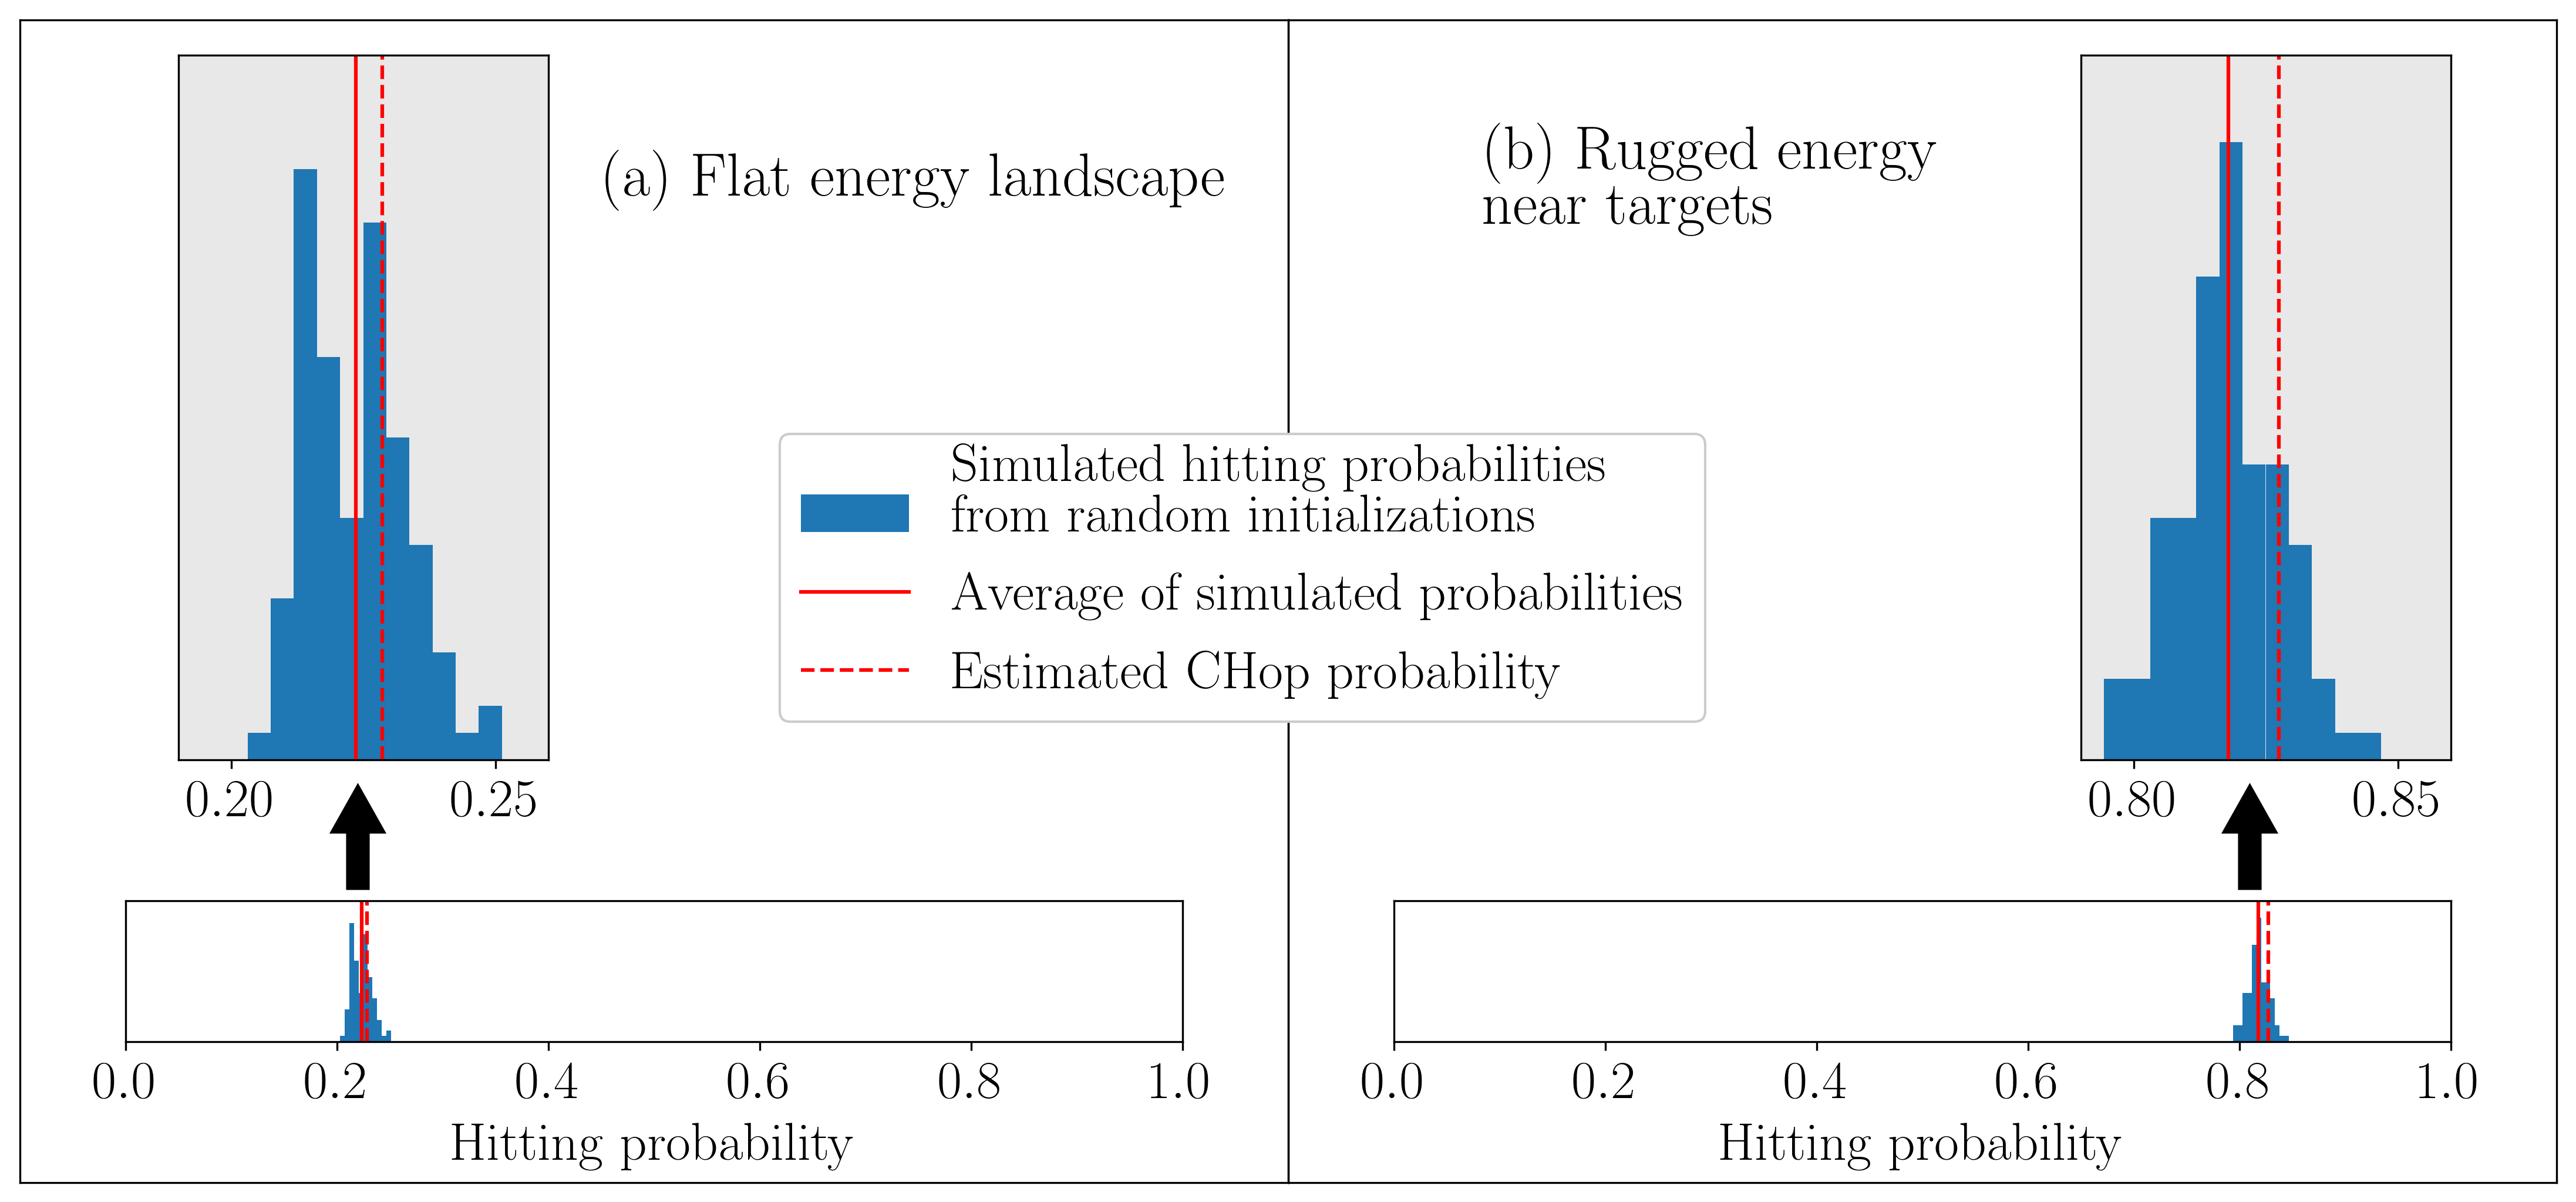
\includegraphics[width=\textwidth]{figs/results.png}
    \caption{\label{fig:results} \textbf{Empirical hitting probabilities from direct simulations vs. CHop probabilities}.  The CHop method accurately answers the question ``where will we go next?'' in the presence of entropic barriers where the targets are small. We start by designating two targets, $A$ and $B$.  For any given initial condition, our task is to determine the probability that we hit $A$ first. We study this question in the context of two different energy landscapes. In subfigure (a), we study the simplest possible case, where we have a flat energy landscape and the dynamics is simply Brownian motion.  In subfigure (b), we consider the case that the energy landscape becomes complicated near the targets.  In both cases we consider 100 random initial locations which are modestly far  away from either target.  For each initial location, we conduct 2000 simulations to estimate the probability of hitting target $A$ first.  For both energy landscapes we see that the hitting probability is approximately constant for initial conditions which are modestly far away from the targets.  Furthermore, the value of this constant is well-approximated by the corresponding CHop probability.  These simulations show that we can use CHop probabilities to accurately approximate the hitting probabilities, even though the CHop probabilities are completely invariant to the energy landscape away from the targets.  Indeed, the CHop probabilities can be computed using only local simulations around the targets, and do not require any simulations that involve the large, flat region between $A$ and $B$.}
\end{minipage}}
\end{figure}

The first set of experiments are ``sanity checks'' designed to show that the CHop method works in the simplest possible case.  For these sanity checks, we work with a flat energy landscape in $\mathbb{R}^5$, where quantities of interest can be obtained in closed form.  In particular, we look at the toy model with parameters $\dimension = 5$ and
\begin{equation*}
x_A = \begin{pmatrix}%
0.5&0.6&0.0&0.0&0.0%
\end{pmatrix},
r_A = 0.02, r_{\tilde{A}} = 0.1
\end{equation*}
for target $A$, and
\begin{equation*}
x_B = \begin{pmatrix}%
-0.7&0.0&0.0&0.0&0.0%
\end{pmatrix},
r_B = 0.04, r_{\tilde{B}} = 0.15
\end{equation*}
for target $B$. Note that because we are working with a flat energy landscape, the values of $d_A, d_B$ won't affect the the results.

\subsubsection{The hitting probabilities are approximately constant}

The first sanity check tests the idea of CHop at its most basic level: that in regions with golf-course potentials, the hitting probabilities are approximately constant for initial conditions that are modestly far away from the targets. In other words, we can establish $\varepsilon$-flatness.  Theorem \ref{thm:epsilon_flat} shows that this must hold in the limiting regime of small $r_A,r_B$ or large $\dimension$, but it is not obvious whether the parameters we use lie in this regime.  

In the toy model, we see that the $\varepsilon$-flatness condition indeed holds, with $\varepsilon \approx 0.0365$.  We ran 2000 diffusion simulations at each of the 100 randomly selected initial conditions in the region $\mathcal{B}(0, 1) \setminus (\tilde{A} \cup \tilde{B})$. This region represents locations that are modestly far away from the targets.  A histogram of these probabilities may be found in Figure \ref{fig:results}.  From this we see that the hitting probabilities are approximately a constant, regardless of the different initial conditions in this region. They all fall in the range of $[0.0820, 0.1185]$.


\subsubsection{The value of this constant is well-approximated using CHop probabilities}

Our second check tests whether the CHop probabilities accurately approximate the hitting probabilities.  For this problem, the relevant CHop probabilities can be computed in closed form:
\begin{equation}
p_A = \frac{\frac{1}{r_A^{2 - \dimension} - r_{\tilde{A}}^{2 - \dimension}}}{\frac{1}{r_A^{2 - \dimension} - r_{\tilde{A}}^{2 - \dimension}} + \frac{1}{r_B^{2 - \dimension} - r_{\tilde{B}}^{2 - \dimension}}}
\end{equation}

According to this formula, the CHop probability is $0.1100$.  This is in good agreement with the average hitting probability $0.0975$ found by direct simulations in the previous section.


\subsubsection{Capacity estimation algorithm}



Finally, we check the accuracy of our capacity estimation algorithm.  We can get an analytical formula for the capacities in this case.  We compare these exact values with those estimated using the method outlined in Section \ref{sec:outlinecapacest}, with parameters $m = 2, n = 4, N_p = 100, N_b = 3, N_s = 1000$ and a time-step of $1 \times 10^{-7}$.  We obtain the following results:

\begin{itemize}
\item $\capac{A}{\tilde{A}}= 0.000637 $, and our method obtained the estimate $0.000591$ 
\item $\capac{B}{\tilde{B}}= 0.005151 $, and our method obtained the estimate $0.004827$ 
\end{itemize}

These show good agreement between the truth and our estimates.

\subsection{Results on Nontrivial Energy Landscape}




In this section, we apply the CHop method to a model with a nontrivial energy landscape around the targets. We see that our algorithm can accurately estimate the hitting probabilities while maintaining great advantage over the direct simulations in terms of speed.

We experimented with the toy model parameters with $\dimension = 5$ and
\begin{equation*}
x_A = \begin{pmatrix}%
0.5&0.6&0.0&0.0&0.0%
\end{pmatrix},
r_A = 0.02,
d_A = 0.05,
r_{\tilde{A}} = 0.1
\end{equation*}
for target $A$, and
\begin{equation*}
x_B = \begin{pmatrix}%
-0.7&0.0&0.0&0.0&0.0%
\end{pmatrix},
r_B = 0.04,
d_B = 0.075,
r_{\tilde{B}} = 0.15
\end{equation*}
for target $B$. We refer the reader to Appendix \ref{sec:energy_function} for more details on the energy used.

\subsubsection{The hitting probabilities are approximately constant}

We again start by testing the basic idea of CHop: we use direct simulations to test that the hitting probabilities are approximately constant for initial conditions that are modestly far away from the targets.  The results can be seen in Figure \ref{fig:results}.   For every initial condition we tested, we found that the hitting probability fell in the interval $[0.7985, 0.8460]$, suggesting that the $\varepsilon$-flatness condition holds with $\varepsilon \approx 0.0475$.



\subsubsection{The value of this constant is well-approximated using CHop probabilities}

Using our capacity estimation algorithm from Section \ref{sec:outlinecapacest}, we obtained an estimate of $0.8360$ for the CHop probability of this model.  This is in good agreement with the average hitting probability $0.8175$ found in our direct simulations.  For the capacity estimation algorithm, we used the parameters $ m = 2, N_p = 3000, N_b = 5, N_s = 1000$ and a time-step of $1 \times 10^{-6}$.  For target $A$ we used $n = 4$ and for the slightly larger target $B$ we used $n = 5$.  

\subsubsection{Capacity estimation algorithm}

In this case it is difficult to assess the accuracy of our capacity estimation algorithm.  It is not possible to obtain exact values for the capacity.  Therefore, we cannot directly test whether our algorithm is accurately estimating the capcities.  However, as the last section showed, the CHop probabilities computed from our estimated capacities do seem to accurately reflect the true hitting probabilities.  This offers some limited evidence that the estimated capacities are also accurate.

We can also test the speed of our capacity estimation algorithm.  We compared the time it takes to estimate the hitting probabilities using direct simulations with the time our capacity estimation algorithm needs to estimate the capacities for all targets. Note that in order to make the direct simulations feasible for the $5$-dimensional toy model we are working on, we made our best effort to make the direct simulation fast.  We used an efficient walk-on-spheres method to simulate trajectories in the flat region,\cite{bingham1972random} JIT compilation to remove loop overhead, multi-CPU parallization, and a relatively coarse time step.  The CPU times for direct simulations and the CHop method are shown below:

\begin{description}
\item[Direct simulation] 33340.36 seconds (4167.55 seconds on an c5d.2xlarge AWS EC2 instance, which has 8 CPUs).  This quantity is an average of the amount of time it took to run 2000 simulations for each of the 100 different initial locations, using a relatively coarse time step of $1 \times 10^{-5}$.  These direct simulations are trivial to perform in parallel, assuring us that there was no significant overhead due to the parallelization.

\item[CHop speed] 50.31 seconds on a single CPU. In doing this we employed a more accurate time step than the one used for direct simulations (i.e.\ a time step of $1 \times 10^{-6}$). Despite this, the CHop method was 82 times faster on a single CPU than the direct simulations on 8 CPUs.

\end{description}

This reflects a 662-fold acceleration. The times reported above reflect a particular choice of parameters, but we found that the accuracy of the algorithm was fairly robust to choices of $m, n, N_p, N_b$ and $N_s$, as long as they are reasonably large. Furthermore note that the time-consuming elements of our capacity estimation algorithm are ``embarassingly parallelizable'' and it should be easy to further accelerate our capacity estimation algorithm using parallelization.  There was no need to do so in this case because we could easily run the CHop method on our laptops.  However, larger scale problems would certainly benefit from this kind of additional acceleration.
\section{Conclusions and Discussions}\label{sec:discussion}

In this work, we offer new insights in the presence of entropic barriers, from a hitting-probability perspective. While lacking timing information, hitting probabilities offer more kinetic understanding than purely thermodynamic analyses, and appear as an important subproblem in various other methods. We show that hitting probabilities, in the presence of entropic barriers where targets are small, often feature an approximate invariance to initial conditions away from the targets. This invariance further imply an invariance to the energy landscape away from the targets. This means that the hitting probabilities can be calculated using only local simulations around the targets. These insights are used to develop CHop, an practical algorithm to estimate hitting probabilities of small targets in the presence of entropic barriers. Numerical experiments on a prototypical entropic barrier, a toy model with a golf-course potential, demonstrate the effectiveness of CHop.

Entropic barriers, which arise because of the difficulty of reaching a small number of target configurations out of a vast number of possible configurations, are in contrast to \emph{enthalpic barriers}, which arise because of the diffuculty of escaping local minima. The challenges of molecular dynamics result from the complicated energy landscapes associated with different biomolecular systems, and can largely be summarized by these two different kinds of barriers. However, careful inspection of the existing methods shows that a majority of the previous developments focus on enthalpic barriers, where the central picture consists of an energy landscape with a multitude of local minima separated by high energetic barriers. A less studied picture involves the entropic barriers, where the energy landscapes has essentially no local minima, and the main difficulty is in finding small targets. We hope this work provides valuable insights into this important but less studied picture, and that it sheds some light into the broader problem of understanding the role of entropy in the kinetics of complex biomolecular systems. 

Our interests in this work come from thinking about RNA folding, and we see this work as laying the foundation for a general-purpose method for the folding of RNA molecules. The central picture is that of a hierarchical golf course: each part of the configuration space that are consistent with a particular secondary structure can be thought of as a golf course; the ``holes" in this golf course are other secondary structures obtained by forming new base pairs; breaking base pairs would bring us back to a larger golf course, while forming base pairs would bring us into a smaller one. CHop would serve as a fundamental tool in this picture. This is an ambitious proposal, and opens all kinds of interesting questions involving the geometry of the configuration space and the folding dynamics. Furthremore, under this picture, in addition to hitting probabilities, CHop can provide us with more kinetic information of the system, by giving us a way to efficiently get sequences of secondary structures. These sequences can play an important role in understanding questions like important intermediates and folding pathways of non-coding RNA molecules.

\newpage

\appendix

%     _    ____  ____  _____ _   _ ____ _____  __     _    
%    / \  |  _ \|  _ \| ____| \ | |  _ \_ _\ \/ /    / \   
%   / _ \ | |_) | |_) |  _| |  \| | | | | | \  /    / _ \  
%  / ___ \|  __/|  __/| |___| |\  | |_| | | /  \   / ___ \ 
% /_/   \_\_|   |_|   |_____|_| \_|____/___/_/\_\ /_/   \_\
                                                         


\section{Stationary Reversible Diffusion Processes}\label{sec:reversible_diffusion}

In this section, we set notation and review known properties of stochastic differential equations.   

\subsection{Defining the process}

Let $\dimension \geq 3$ and $\Omega \subset \mathbb{R}^\dimension$ be a bounded open set with smooth boundary.  Our central object of interest will be a diffusion $X$ trapped in $\Omega$ by some kind of reflecting boundaries.  The construction of such reflected diffusions is a bit of a delicate art, so we will start by taking a moment to rigorously define the process $X$.

Let $W$ denote a Brownian motion.  Let $b:\ \bar \Omega \rightarrow \mathbb{R}^\dimension,\sigma:\ \bar \Omega \rightarrow \mathbb{R}^{\dimension\times\dimension}$ smooth.  Let $\mathbf{n}$ denote the outward normal of $\partial \Omega$ and $\nu:\ \partial \Omega \rightarrow \mathbb{R}^\dimension$ a smooth vector field satisfying $\mathbf{n}^T\nu\geq c>0$. Let $x_0 \in \Omega$.  Then there is a pathwise unique continuous $W$-adapted strong Markov process $X$ and (random) measure $L$ such that 
\begin{gather}\label{eq:SDER}
X_t = x_0 + \int_0^t b(X_s)ds + \int_0^t \sigma(X_s)dW_s - \int_0^t \nu(X_s) L(ds)
\end{gather}
and $L(\{t:\ X_t \notin \partial \Omega\})=0$.\cite{lions1984stochastic} 

We will further assume that $X$ is reversible with respect to a measure $\rho(dx)=e^{-U(x)}dx$ with $\rho(\Omega)=1$ and $U:\ \bar \Omega \rightarrow \mathbb{R}$ smooth.  Here by reversible we mean that
\[
\int_{A}\mathbb{P}(X_{t}\in B|X_{0}=x)\rho(dx)  =\int_{B}\mathbb{P}(X_{t}\in A|X_{0}=x)\rho(dx)
\]
for any open sets $A,B\subset \Omega$ and any $t>0$.  Due to this condition, we are not completely free in our choice of $b,\sigma,\nu$.  A sufficient condition for reversibility is $X$ is given in Chen,\cite{chen1993reflecting} namely that
\begin{align*}
b_i(x)&=\frac{1}{2} \sum_j \partial a_{ij}(x)/\partial x_j - \frac{1}{2}\sum_j a_{ij}(x) \partial U(x)/\partial x_j \\
\nu(x)&= a(x) \mathbf{n}(x)
\end{align*}
where $a=\sigma\sigma^T$ is uniformly elliptic.  Specifically, Chen shows that under these conditions, one can construct a reversible continuous $W$-adapted strong Markov process which also obeys Equation (\ref{eq:SDER}).  Since Lions\cite{lions1984stochastic} showed that the solution to Equation (\ref{eq:SDER}) is unique, it follows that Chen's process is exactly $X$.  Thus, since Chen's process is reversible, $X$ must also be reversible.  It seems that the conditions on $b,\nu$ are in fact necessary for reversibility, although our review of the literature did not reveal a conclusive answer.  Proposition 4.5 of Pavliotis\cite{Pavliotis2016-xn} gives a formal argument in this direction, but we could not find a completely rigorous analysis.  The results of this paper apply only to reversible processes for which these $b,\nu$ conditions hold.

\subsection{Three perspectives on hitting probabilities}

Many of our results are based on the fact that hitting probability functions can actually be seen from three distinct perspectives:

\begin{enumerate}
    \item Hitting probabilities.  Let $\tau_S \triangleq \inf\{t:\ X_t \in S\}$ for any set $S$ and $h_{A,B}(x) \triangleq \mathbb{P}(X_{\tau_{A\cup B}}\in \partial A)$.
    
    \item Dirichlet problem.  Let $h^\mathrm{dir}_{A,B}(x)$ denote the solution to the partial differential equation
    \begin{align*}
    0 &= \sum_{i = 1}^\dimension b_i (x) \frac{\partial u
        (x)}{\partial x_i} + \frac{1}{2} \sum_{i = 1}^\dimension \sum_{j = 1}^\dimension a_{ij} (x)
        \frac{\partial^2 u (x)}{\partial x_i \partial x_j}\\
    1 &= u(x),x\in A \\
    0 &= u(x) ,x\in B \\
    0 &= \mathbf{n}(x)^Ta(x)\nabla u(x), x \in \partial{\Omega} \backslash (\partial A \cup \partial B)
    \end{align*}
    This solution is unique and smooth.\cite{lieberman1986mixed}  What's more, it is equal to the hitting probability function: $h^\mathrm{dir}_{A,B}(x)=h_{A,B}(x)$ (cf.\ Section 6.7 of Chen\cite{chen2012symmetric}).

    \item Variational form.  Let $\mathscr{E}(f,g)\triangleq \int_\Omega \nabla f(x)^T a(x) g(x) \rho(dx)$ denote the ``Dirichlet Form.''  Let $\mathscr L^2(\bar \Omega,\rho)$ denote the Hilbert space of functions on $\bar \Omega$ which are square-integrable with respect to $\rho$.  Let $\mathcal{H}^1(\bar \Omega,\rho)=W^{1,2}(\bar \Omega,\rho) \subset \mathscr{L}^2(\bar \Omega,\rho)$ denote the corresponding once-weakly-differentiable Hilbert Sobolev space.  Let $A,B\subset \Omega$, disjoint, and let $h^\mathrm{var}_{A,B}(x)$ denote the solution to 
    \begin{align*}
    \min_{u \in \mathcal H^1} \quad & \mathscr{E}(u,u) \\
    \mbox{subject to} \quad & u(x)\geq1,x\in A \\
     & u(x)\leq0,x\in B
    \end{align*}
    This solution is unique and equal to $h^\mathrm{dir}$.\cite{karatson2005discrete}  We will call the value of $\mathscr{E}(h^\mathrm{var}_{A,B}(x),h^\mathrm{var}_{A,B}(x))$ the ``condensor capacity'' from $\partial A$ to $\partial B$, or just the ``capacity'' for short.  We will denote it by $\capac{A}{\Omega \backslash B}$.
\end{enumerate}


  We will use all three of these perspectives to show our results.  For example, consider how these different perspectives help us show the following:

\begin{proposition}\label{prop:capacity}
Let $A\subset \tilde A,B\subset \tilde B$ with $\tilde A,\tilde B$ disjoint.  Then 
\[
\capac{A\cup B}{\tilde A \cup \tilde B}=\capac{A}{\tilde A}+\capac{B}{\tilde B}
\]
\end{proposition}
\begin{proof}
Since $\tilde A,\tilde B$ are disjoint and $X$ is continuous, the process cannot cross from one to the other without hitting the boundary.  Thus we have $\tau_{\partial \tilde A\cup \partial \tilde B \cup \partial A \cup \partial B}=\tau_{\partial \tilde A \cup \partial A}$ as long as $X_0\in\tilde A$.  We get a symmetric result if $X_0\in \tilde B$.  If $X_0\notin \tilde A,\tilde B$, then trivially we see that $h_{A\cup B,(\tilde A \cup \tilde B)^c}(x)=0$.  It follows that
\[
h_{A\cup B,(\tilde A\cup\tilde B)^c}(x) = 
    \begin{cases}
    h_{A,\tilde A}(x) & \mbox{if }x\in \tilde A\\
    h_{B,\tilde B}(x) & \mbox{if }x\in \tilde B\\
    0 & \mbox{if }x\notin \tilde A\cup\tilde B
    \end{cases}
\]
We can now use this probabilistic perspective to help us understand the capacity by articulating it as the Dirichlet form on the relevant hitting probability functions
\begin{align*}
\capac{A\cup B}{\tilde A \cup \tilde B} &= 
        \int_{\tilde A} h_{A,\tilde A}dx
        +\int_{\Omega\backslash \tilde A \cup \tilde B} 0 dx  
        +\int_{\tilde B} h_{B,\tilde B}dx \\
        &= \capac{A}{\tilde A}+\capac{B}{\tilde B}
\end{align*}
as desired.
\end{proof}


%     _    ____  ____  _____ _   _ ____ _____  __  ____  
%    / \  |  _ \|  _ \| ____| \ | |  _ \_ _\ \/ / | __ ) 
%   / _ \ | |_) | |_) |  _| |  \| | | | | | \  /  |  _ \ 
%  / ___ \|  __/|  __/| |___| |\  | |_| | | /  \  | |_) |
% /_/   \_\_|   |_|   |_____|_| \_|____/___/_/\_\ |____/ 
                                                       


\section{Proof of Theorem \ref{thm:main_thm}}\label{sec:proof_thm}

Let $A\subset\tilde A\subset\Omega,B\subset\tilde B\subset\Omega$.  Let $\tilde A,\tilde B$ be disjoint and $\Omega \backslash (\tilde A \cup \tilde B)$ $\varepsilon$-flat for the hitting probabilities $h_{A,B}(x)$.  We assume the set boundaries are all smooth.  

Under these conditions, we will show we can use local capacities to get good approximations for $h_{A,B}(x)$ when $x\notin \tilde A,\tilde B$.  To do so, our key idea is to uncover upper and lower bounds on the value of the Dirichlet form applied to this function, $\mathcal{E}(h_{A,B},h_{A,B})$.  We will see that these bounds can be understood in terms of local capacities, and the resulting inequalities will then yield our main result in the form of Theorem \ref{thm:main_thm}.

\begin{lemma}  The Dirichlet form of $h_{A,B}$ can be upper-bounded in terms of the capacities:
\[ \mathcal{E} (h_{A,B}, h_{A,B}) \leqslant \frac{\tmop{cap} (A, \tilde{A}) \tmop{cap} (B,
\tilde{B})}{\tmop{cap} (A, \tilde{A}) + \tmop{cap} (B, \tilde{B})} \]
\end{lemma}
\begin{proof}
We recall from Appendix \ref{sec:reversible_diffusion} that
%
\[
\mathcal{E} (h_{A,B}, h_{A,B}) = \capac{A}{B^c} \leq \mathcal{E} (u,u)
\]
%
for any $u$ with $u(A)\geq1,u(B)\leq0$.  Thus, to prove an upper bound it suffices to find any such function for which we can calculate $\mathcal{E}(u,u)$.  To this end, consider
%
\[
u_c (x) \triangleq \left\{ \begin{array}{ll}
(1 - c) h_{A, \widetilde{A}^c} (x) + c & \tmop{if} x \in \tilde{A}\\
c (1 - h_{B, \widetilde{B}^c} (x)) & \tmop{if} x \in \tilde{B}\\
c & \tmop{otherwise}
\end{array} \right. 
\]
%
These functions are well-suited to giving us upper bounds on $\mathcal{E} (h_{A,B}, h_{A,B})$.  Indeed:
\begin{itemize}
\item $u_c(A)=1,u_c(B)=0$.  Indeed, $u_c$ takes a constant value $c$ outside of $\tilde A,\tilde B$, drops smoothly in $\tilde B$ to achieve 0 on $\partial B$, and rises smoothly in $\tilde A$ to achieve 1 on $\partial \tilde A$.  
\item Noting that $u_c$ is written as a piecewise combination of hitting probability functions, we see that its Dirichlet form can be calculated in terms of capacities on local regions: $\mathcal{E}(u_c,u_c) = (1 - c)^2 \tmop{cap} (A, \tilde{A}) + c^2 \tmop{cap} (B, \tilde{B})$.
\end{itemize}
Thus the $u_c$ functions give us a practical way to calculate upper bounds: 
\[
\mathcal{E} (h_{A,B}, h_{A,B})\leq (1 - c)^2 \tmop{cap} (A, \tilde{A}) + c^2 \tmop{cap} (B, \tilde{B})
\]
This inequality holds for any value of $c$.  To get the best bound, we can take derivatives to minimize the right hand side with respect to $c$.  The result is 
\[
c^* = \frac{\capac{A}{\tilde A}}{\capac{A}{\tilde A}+\capac{B}{\tilde B}}
\]
Plugging this into the previous equation, we obtain our final result.
\end{proof}

%%%%%%%%%%%
%%%%%%%%%%%

\begin{lemma}  Let $m = \frac{1}{2} (\sup_{x \notin \tilde A,\tilde B} h_{A,B} (x) + \inf_{x \notin \tilde A,\tilde B} (h_{A,B} (x)))$.  The Dirichlet form of $h_{A,B}$ can be lower-bounded in terms of $m$ and the capacities:
\[\mathcal{E} (h_{A,B}, h_{A,B}) \geq  
   \left( 1 - m - \frac{\varepsilon}{2} \right)^2 \tmop{cap} (A,\tilde{A}) \indicatorf{m\leq 1-\frac{\varepsilon}{2}} + 
   \left( m- \frac{\varepsilon}{2} \right)^2 \tmop{cap} (B, \tilde{B})\indicatorf{m\geq \frac{\varepsilon}{2}} 
\]
\end{lemma}
\begin{proof}
Recall that $\mathcal{E} (h_{A,B}, h_{A,B})$ can be expressed as an integral over $\Omega$.  We decompose this into three integrals: one over $\tilde A$, one over $\Omega \backslash \tilde A,\tilde B$, and one over $\tilde B$.  
\[
\mathcal{E} (h_{A,B}, h_{A,B}) = \int_{\tilde A} \Vert \sigma \nabla h_{A,B}\Vert^2 dx
                                 + \int_{\tilde B} \Vert \sigma \nabla h_{A,B}\Vert^2 dx
                                 + \int_{\Omega \backslash \tilde A,\tilde B} \Vert \sigma \nabla h_{A,B}\Vert^2 dx
\]
Since the integrand is always positive, we can get a lower bound by simply ignoring the integral over $\Omega \backslash \tilde A,\tilde B$ and focusing on the integrals over $\tilde A,\tilde B$.  The $\tilde A,\tilde B$ integrals can be lower-bounded using capacities.  

For example, let us focus on the $A$ case.  There are two different possibilities we must consider:
\begin{itemize}
\item If $m>1-\varepsilon/2$ we will simply note that the integral over the $\tilde A$ region is nonnegative.  
\item If $m\leq 1-\varepsilon/2$, then we define
    \[
    u_A (x) \triangleq \frac{h_{A,B} (x) - m - \frac{\varepsilon}{2}}{1 - m - \frac{\varepsilon}{2}}
    \]
    Note that $u_A(A)\geq1,u_A(\tilde A)\leq 0$.  Indeed, $h_{A,B}(x)=1$ for $x \in \partial A$ and the $\varepsilon$-flatness condition shows that $h_{A,B}(x) \leq m + \frac {\varepsilon}{2}$ for $x \in \partial \tilde A$.  Thus, applying the definition of the capacity, we see that $\mathcal{E}(u_A,u_A) \geq \capac{A}{\tilde A}$.  Thus we see that
    %
    \begin{align*}
    \int_{\tilde A} \Vert \sigma \nabla h_{A,B}\Vert^2 dx &= \left(1 - m - \frac{\varepsilon}{2}\right)^2 \int_{\tilde A} \Vert \sigma \nabla u_{A}\Vert^2 dx\\
         &\geq \left(1 - m - \frac{\varepsilon}{2}\right)^2 \capac{A}{\tilde A}
    \end{align*}
\end{itemize}
Putting these together, we obtain
\[
\int_{\tilde A} \Vert \sigma \nabla h_{A,B}\Vert^2 dx \geq \left(1 - m - \frac{\varepsilon}{2}\right)^2 \capac{A}{\tilde A}\indicatorf{m\leq 1-\frac{\varepsilon}{2}}
\]
Applying the same ideas to the integral over $\tilde B$, we obtain our result.
\end{proof}

%%%%%%%%%%%
%%%%%%%%%%%

We are now in a position to prove Theorem \ref{thm:main_thm} from the main text:

\begingroup
\def\thetheorem{\ref{thm:main_thm}}
\begin{theorem}  The hitting probabilities can be well-approximated by the capacities:
\[ \sup_{x \notin \tilde A,\tilde B} \left| h_{A,B} (x) - \frac{\ensuremath{\operatorname{cap}} (A,
\tilde{A})}{\ensuremath{\operatorname{cap}} (A, \tilde{A})
+\ensuremath{\operatorname{cap}} (B, \tilde{B})} \right| \leqslant \varepsilon + \sqrt{\varepsilon/2} \]
\end{theorem}
\addtocounter{theorem}{-1}
\endgroup

\begin{proof}
\newcommand{\capA}{\kappa_A}
\newcommand{\capB}{\kappa_B}

To simplify notation, let $\capA=\capac{A}{\tilde A}$ and $\capB=\capac{B}{\tilde B}$.  Applying the previous two lemmas together, we obtain the inequality
\[
\frac{\capA \capB}{\capA +\capB}
\geq \mathcal{E}(h_{A,B},h_{A,B}) \geq
\left( 1 - m - \frac{\varepsilon}{2} \right)^2 \capA \indicatorf{m\leq 1-\frac{\varepsilon}{2}} + 
   \left( m- \frac{\varepsilon}{2} \right)^2 \capB \indicatorf{m\geq \frac{\varepsilon}{2}} 
\]
where $m = \frac{1}{2} (\sup_{x \notin \tilde A,\tilde B} h_{A,B} (x) + \inf_{x \notin \tilde A,\tilde B} (h_{A,B} (x)))$.  In analyzing this inequality, there are three possibilities to consider.  
\begin{itemize}
    \item If $m \in (\epsilon/2,1-\epsilon/2)$, the quadratic formula yields
    \begin{eqnarray*}
    m & \geqslant & \frac{\capA}{\capA + \capB} + \frac{
    \frac{\varepsilon}{2}(\capB - \capA) - 
    \sqrt{\capA \capB \varepsilon( 2 - \varepsilon)}}{\capA+\capB}\\
    m & \leqslant & \frac{\capA}{\capA + \capB} + \frac{
    \frac{\varepsilon}{2}(\capB - \capA) +
    \sqrt{\capA \capB \varepsilon( 2 - \varepsilon)}}{\capA+\capB}
    \end{eqnarray*}
    Applying $\left|\frac{\capB - \capA}{\capA + \capB}\right| \leq 1$ and the fact that the geometric mean $\sqrt{\capA \capB}$ never exceeds the arithmetic mean $(\capA+\capB) / 2$, it follows that
    \[
    \left|m -  \frac{\capA}{\capA + \capB}\right| \leq \frac{\epsilon +\sqrt{\epsilon (2-\epsilon)}}{2}
    \]
    Applying the fact that $m$ was designed so that $|h_{A,B}(x) - m| <\varepsilon/2$ for all $x \notin \tilde A,\tilde B$, we obtain
    \[
    \left|h_{A,B}(x) -  \frac{\capA}{\capA + \capB}\right| \leq \frac{2\epsilon +\sqrt{\epsilon (2-\epsilon)}}{2}
    \]

    \item If $m<\varepsilon/2$, our equations become 
    \[
    \frac{\cancel{\capA} \capB}{\capA +\capB}
    \geq
    \left( 1-m- \frac{\varepsilon}{2} \right)^2 \cancel{\capA} 
    \]
    Our assumption that $m \leq \varepsilon/2$ indicates that $(1- m- \varepsilon/2)^2 \geq (1-\varepsilon)^2$, thus in fact we have 
    \[
    \frac{\capB}{\capA +\capB}
    \geq
    \left( 1- \varepsilon \right)^2  = 1 + \varepsilon^2 - 2\varepsilon
    \]
    which means that $\capA/(\capA +\capB)
    \leq
    2\varepsilon - \varepsilon^2 \leq 2\varepsilon$.  
    Thus we assumed $m\in[0,\varepsilon/2]$ and showed that $\capA/(\capA+\capB)\in[0,2\varepsilon-\varepsilon^2]$, so it follows that 
    \[
    \left|m -  \frac{\capA}{\capA + \capB}\right| \leq 2\varepsilon -\varepsilon^2
    \]
    and so for any $x\notin \tilde A,\tilde B$, we have 
    \[
    \left|h_{A,B}(x) -  \frac{\capA}{\capA + \capB}\right| \leq 2.5\varepsilon -\varepsilon^2
    \]
    
    \item If $m>1-\varepsilon/2$, the same bound can be achieved by arguments which are symmetric to those employed in $m<\varepsilon/2$:
    \[
    \left|h_{A,B}(x) -  \frac{\capA}{\capA + \capB}\right| \leq 2.5\varepsilon -\varepsilon^2
    \]
\end{itemize}
Our final result is found by noting that all these bounds are upper-bounded by $\varepsilon + \sqrt{\varepsilon/2}$.
\end{proof}

%     _    ____  ____  _____ _   _ ____ _____  __   ____ 
%    / \  |  _ \|  _ \| ____| \ | |  _ \_ _\ \/ /  / ___|
%   / _ \ | |_) | |_) |  _| |  \| | | | | | \  /  | |    
%  / ___ \|  __/|  __/| |___| |\  | |_| | | /  \  | |___ 
% /_/   \_\_|   |_|   |_____|_| \_|____/___/_/\_\  \____|
           

\section{Proof of Theorem \ref{thm:epsilon_flat}}\label{sec:proof_epsilon_flat}

Consider the setup of the Toy Model described in Section \ref{sec:toy_model}.  A stationary reversible diffusion $X$ is trapped inside the unit $\dimension$-dimensional ball.  We are interested to know which target $X$ will hit first: $A=\bb{x_A,r_A}$ or $B=\bb{x_B,r_B}$.  The function $h_{A,B}(x)$ indicates the probability we will hit $A$ first if $X_0=x$.  We will be particularly interested in the case where $X_0$ is outside of $\tilde A=\bb{x_A,r_{\tilde A}},\tilde B=\bb{x_A,r_{\tilde B}}$.  Also recall that in the toy example the diffusion behaves as a Brownian motion outside of $\dot A=\bb{x_A,d_A},\dot B=\bb{x_B,d_B}$.  

It turns out that by taking the $\dimension$ is sufficiently high or $d_A,d_B$ are sufficiently small, we can make the hitting probabilities arbitrarily close to constant in the region away from $\tilde A,\tilde B$.  This is the content of Theorem \ref{thm:epsilon_flat} from the main text, which we restate here for the convenience of the reader:

\begingroup
\def\thetheorem{\ref{thm:epsilon_flat}}
\begin{theorem}  For any fixed value of the ambient dimension $\dimension \geq 3$ and any $r_{\tilde{A}}, r_{\tilde{B}}, \varepsilon > 0$, there exists a constant $c=c(\dimension, r_{\tilde{A}}, r_{\tilde{B}}, \varepsilon)$ such that if $d_{A}, d_{B} < c$ then $\bb {0, 1} / (\tilde{A} \cup \tilde{B})$ is $\varepsilon$-flat for the function $h_{A,B}(x)$.  Likewise for any fixed value of $d_{A}, r_{\tilde{A}}, d_{B}, r_{\tilde{B}}, \varepsilon>0$, there exists a constant $c=c(d_{A}, r_{\tilde{A}}, d_{B}, r_{\tilde{B}}, \varepsilon)$ such that if $\dimension \geq c$ then $\bb {0, 1} / (\tilde{A} \cup \tilde{B})$ is $\varepsilon$-flat for the function $h_{A,B}(x)$.
\end{theorem}
\addtocounter{theorem}{-1}
\endgroup

\begin{proof}
Let us assume $X_0 \notin \tilde A,\tilde B$.  There are essentially two things that must be proved:
\begin{enumerate}
\item The process $X$ converges to its stationary distribution fairly quickly.  This is supported by Lemma \ref{lem:uniform_ergodicity}.  Since $h_{A,B}(x) \in [0,1]$, this Lemma gives that
%
\[
|\mathbb{E}[h_{A,B}(M_t)-h_{A,B}(Z)]| \leq 2^2/4t =1/t
\]
%
where $Z$ is distributed according to the uniform distribution on $\Omega$ and $M$ is a Brownian motion trapped in $\Omega$ by normally reflecting boundaries.  

To connect this result on $M$ to our object of interest $h_{A,B}$, note that without loss of generality we may assume $X,M$ are on the same probability space and $M_t=X_t$ for $t<\tilde\tau \triangleq \inf \{t:\ X_t \in \partial \dot A \cup \partial \dot B\}$.  Moreover, noting that $\tilde\tau\wedge t$ is a stopping time and applying the Strong Markov property, we observe that 
%
\[
h_{A,B}(x) = \mathbb{E} [\indicatorf{X_{t\wedge\tilde\tau} \in \partial A}] 
        = \mathbb{E} [\mathbb{E}[\indicatorf{X_{t\wedge\tilde\tau} \in \partial A} | X_{t\wedge\tilde\tau}]]
        = \mathbb{E} [h_{A,B}(X_{t\wedge\tilde\tau})] = \mathbb{E} [h_{A,B}(M_{t\wedge\tilde\tau})]
\]
%
Thus
\begin{align*}
|h_{A,B}(x) - \mathbb{E}[h_{A,B}(Z)]| &= |\mathbb{E} [h_{A,B}(M_{t\wedge\tilde\tau})] - \mathbb{E}[h_{A,B}(Z)]|\\
&\leq |\mathbb{E} [h_{A,B}(M_{t\wedge\tilde\tau})] - h_{A,B}(M_t)]| + |\mathbb{E} [h_{A,B}(M_{t}) - h_{A,B}(Z)]|\\
&\leq \mathbb{P}(\tilde \tau \leq t) + 1/t
\end{align*}
%

\item The hitting time $\tilde \tau$ is generally long.  This is supported by Lemma \ref{lem:longtime}, which says that if $X_0 \not\in\tilde{A} \cup \tilde{B}$ we can ensure
%
\[
\mathbbm{P} \left( \tilde{\tau} \leq t \right) < \varepsilon/2
\]
%
for arbitrarily small $\varepsilon$ and arbitarily large $t$, by taking $\dimension$ sufficiently high or $d_A,d_B$ sufficiently small.
\end{enumerate}
Putting these two results together at $t=2/\varepsilon$ we obtain that we can make $|h_{A,B}(x) - \mathbb{E}[h_{A,B}(Z)]| \leq \varepsilon / 2 + \varepsilon/2 = \varepsilon$ for arbitrarily small $\varepsilon$ by taking $\dimension$ sufficiently high or $d_A,d_B$ sufficiently small.
\end{proof}

%%%%%%%%%%%%%%%%%%%%%%
%%%%%%%%%%%%%%%%%%%%%%

\begin{lemma}
\label{lem:uniform_ergodicity}(Uniform ergodicity) Let $\Omega\subset\mathbbm{R}^d$ be a convex set with diameter $\xi$ and let $M$ denote a Brownian motion trapped by reflecting boundaries inside $\Omega$.  The distribution of $M_t$ converges uniformly to the uniform distribution:
%
\[ 
\sup_{f:\ \Omega\rightarrow [0,1]} | \mathbb{E}[f(M_t) - f(Z)|M_0=x]| \leq \xi^2/4t \qquad \forall x\in \Omega, t>0
\]
%
where $Z$ is uniformly distributed on $\Omega$.
\end{lemma}
\begin{proof}
Let $F_\xi(t)$ denote the survival function for the first exit time of a one-dimensional Brownian motion from the intervals $[-\xi,\xi]$ when initialized at the origin.  Per Loper,\cite{Loper2018} 
\[
\sup_{f:\ \Omega\rightarrow [0,1]} | \mathbb{E}[f(M_t) - f(Z)|M_0=x]| \leq F_\xi(4t)
\]
It is well-known that this one-dimensional first-exit time is characterized by an expected value of $\xi^2$.  Thus, applying the Markov inequality, it follows that $F_\xi(t) \leq \xi^2 / t$ and so $F_\xi(4t) \leq \xi^2 / 4t$. 
\end{proof}

\begin{lemma}
\label{lem:longtime}Let $\tilde{\tau}= \inf \{ t : X_t \in \dot A \cup \dot B\}$. For any fixed value of $\dimension
\geqslant 3$ and $r_{\tilde{A}}, r_{\tilde{B}}, \varepsilon,t > 0$, there
exists some $c (\dimension, r_{\tilde{A}}, r_{\tilde{B}}, \varepsilon,t)$ such that if
$d_A, d_B < c$, then
\[ \mathbbm{P} \left( \tilde{\tau} < t |X_0 \not\in\tilde{A} \cup \tilde{B} \right) < \varepsilon \]
Likewise, for any fixed value of $d_A, r_{\tilde{A}}, d_B, r_{\tilde{B}},
\varepsilon,t > 0$, there exists some $c (d_A, r_{\tilde{A}}, d_B,
r_{\tilde{B}}, \varepsilon,t)$, such that the same property holds as long as $\dimension \geqslant c$.
\end{lemma}

\begin{proof}
Our task is to show that $\tilde \tau$ is large with high probability.  Note that it suffices to show that $\tilde \tau_A \triangleq \inf\{t:\ X_t\in \dot A\}$ and $\tilde \tau_B \triangleq \inf\{t:\ X_t\in \dot B\}$ are both large with high probability and then apply a union bound.  Thus, without loss of generality we will focus on showing that $\tilde \tau_A$ is large with high probability.  For this, Chernoff's bound shows that it would be sufficient to show that we can make
\[
g(x)=\mathbb{E}[e^{-\frac{1}{2}\tilde \tau_A}|X_0=x]
\] 
aribitrarily small for every $x\notin \tilde A$.  Furthermore note that for any $X_0 \notin \tilde A$, the continuity of $X$ dictates that $X$ must cross the set $S=S_{\tilde d_A}=\{x:\ |x-x_A| = \tilde d_A\}$ before $\tilde \tau_A$, as long as $\tilde d_A \in (d_A,r_{\tilde A})$.  Thus, applying the strong Markov property of $X$, we have that $g(x)\leq \sup_{y\in S_{\tilde d_A}}g(y)$ for any $x \notin \tilde A$.

In summary, to prove our theorem it will suffice to show that by taking $d_A$ sufficiently small or $\dimension$ sufficiently large we can ensure that $g(x)$ is uniformly arbitrarily small on $S_{\tilde d_A}$ for some $\tilde d_A \in (d_A,r_{\tilde A})$.  To show this, we will make use of two other hitting probabilities:
\[
T =\inf \{t:\ X_t \notin \tilde A \backslash \dot A\} 
\qquad
T_1 =\inf \{t>T:\ X_t \in S\} 
\]
If $T\neq \tilde \tau_A$, note that the process must cross $S$ again before reaching $\dot A$ and so $T_1 \leq \tilde \tau_A$.  Thus, applying the strong Markov property we see that for any $x\in S$ we have
\begin{align*}
g(x) = &\mathbb{E}[e^{-\frac{1}{2}\tilde \tau_A}\indicatorf{T=\tilde \tau_A}|X_0=x]+
                    \mathbb{E}[e^{-\tilde \tau_A}\indicatorf{T\neq\tilde \tau_A}|X_0=x]\\
     = & \mathbb{E}[e^{-\frac{1}{2}\tilde \tau_A}\indicatorf{T=\tilde \tau_A}|X_0=x]+
                    \mathbb{E}[e^{-T_1}g(X_{T_1})\indicatorf{T\neq\tilde \tau_A}|X_0=x]\\
     \leq & \mathbb{E}[e^{-\frac{1}{2}T}\indicatorf{T=\tilde \tau_A}|X_0=x]+
                    \mathbb{E}[e^{-\frac{1}{2}T}\indicatorf{T\neq\tilde \tau_A}|X_0=x]\left(\sup_{y\in S} g(y)\right)
\end{align*}
Note furthermore that the law of $e^{-\frac{1}{2}T},\indicatorf{T=\tilde \tau_A}$ is actually the same for every $x\in S$, due to the fact that the diffusion behaves simply like a Brownian motion inside $\tilde A \backslash \dot A$ and the law of $T,\indicatorf{T=\tau_A}$ are thus functions of the one-dimensional diffusion of $|X_t-x_A|$.  In fact, Wendel\cite{Wendel1980-sj} gives explicit formulas for $\mathbb{E}[e^{-\frac{1}{2}T}\indicatorf{T=\tilde \tau_A}|X_0=x],\mathbb{E}[e^{-\frac{1}{2}T}\indicatorf{T\neq\tilde \tau_A}|X_0=x]$ which depend only upon $|x-x_A|,r_{\tilde{A}},d_A$.  Applying this, taking the supremum over $x$ of our previous formula, and rearranging, we obtain
\begin{align*}
\sup_{x\in S} g(x) &\leq \frac{\mathbb{E}[e^{-\frac{1}{2}T}\indicatorf{T=\tilde \tau_A}|X_0\in S]}{1-\mathbb{E}[e^{-\frac{1}{2}T}\indicatorf{T\neq\tilde \tau_A}|X_0\in S]} \triangleq L(d_A,\tilde d_A,r_{\tilde A},\dimension)
\end{align*}
Applying Wendel's formulas, we obtain a closed form expression for $L$:
\[
=\frac{\left( \frac{d_A}{\tilde{d}_A} \right)^h (I_h (
r_{\tilde{A}}) K_h ( \tilde{d}_A) - I_h ( \tilde{d}_A) K_h (
r_{\tilde{A}}))}{
    \left( \frac{I_h ( r_{\tilde{A}})}{I_h ( \tilde{d}_A)} - \left(
\frac{r_{\tilde{A}}}{\tilde{d}_A} \right)^h  \right)
K_h ( d_A) I_h ( \tilde{d}_A)+ 
    \left( \left( \frac{r_{\tilde{A}}}{\tilde{d}_A}
\right)^h  - \frac{K_h ( r_{\tilde{A}})}{K_h ( \tilde{d}_A)} \right) I_h (d_A)K_h ( \tilde{d}_A)}\\
\]
where $h=(\dimension-2)/2$ and $I_h,K_h$ represent modified Bessel functions of the first and second kind of order $h$.  
 
Thus, to complete our proof, it suffices to show that we can drive $L(d_A,r_{\tilde A},\dimension)$ to zero by taking $d_A$ small or $\dimension$ large:
\begin{itemize}
    \item When $d_A$ is small.  The numerator of $L$ converges to zero as $d_A\rightarrow 0$, because $\frac{d_A}{\tilde{d}_A}\rightarrow 0,h>0$ and the other terms are constant.  On the other hand, the denominator explodes, because as $d_A\rightarrow0$ we have
    \begin{align*}
    & \left( \frac{I_h ( r_{\tilde{A}})}{I_h ( \tilde{d}_A)} - \left(\frac{r_{\tilde{A}}}{\tilde{d}_A} \right)^h  \right)
                K_h ( d_A) I_h ( \tilde{d}_A) \rightarrow +\infty \\
    & \left( \left( \frac{r_{\tilde{A}}}{\tilde{d}_A}\right)^h  - \frac{K_h ( r_{\tilde{A}})}{K_h ( \tilde{d}_A)} \right) 
                I_h (d_A)K_h ( \tilde{d}_A)\rightarrow 0
    \end{align*}
    These limits follow immediately from three properties of Bessel functions:
    \begin{itemize}
        \item $K_h(x)\rightarrow \infty,I_h(x)\rightarrow 0$ as $x\rightarrow 0$ for $h>0$
        \item $K_h(x),I_h(x)>0$ for $x>0,h>0$
        \item $\frac{I_{h}(y)}{I_{h}(x)} > \left(\frac{y}{x}\right)^{h}$ for $y>x$ and $h>0$
    \end{itemize} 
    The first two properties are well-known and can be found in DLMF; the second can be found in Baricz.\cite{noauthor_undated-ti,baricz2010bounds}  In conclusion, since the numerator vanishes and the denominator explodes, we have that overall $L$ vanishes.  
    \item When $\dimension$ is large.  It is clear that the previous result holds for any value of $\tilde d_A\in (d_A, r_{\tilde A})$.  For the large-$\dimension$ case, we will be more picky: we will take $\tilde d_A=\sqrt{d_A r_{\tilde A}}$.  

    Let us look at the numerator first.  Asymptotics from the DLMF give that as $h=(\dimension-2)/2 \rightarrow \infty$ we have
    \begin{align*}
    I_h(x) \sim x^h/2^hh! & & K_h(x) \sim 2^hh!/(2h)x^h  
    \end{align*}
    Here by $f_1(h)\sim f_2(h)$ we mean ``asymptotic equivalence,'' i.e.\ $\lim_{h\rightarrow\infty}f_1(h)/f_2(h)=0$.    Applying to our case:
    \begin{align*}
        \left(\frac{d_A}{\tilde{d}_A}\right)^h I_h (r_{\tilde{A}}) K_h ( \tilde{d}_A) &
                \sim \left(\frac{r_{\tilde{A}} d_A}{\tilde{d}_A^2}\right)^h/2h \rightarrow 0 \\
        \left(\frac{d_A}{\tilde{d}_A}\right)^h I_h ( \tilde{d}_A) K_h (r_{\tilde{A}}) &
                \sim \left(\frac{ d_A}{r_{\tilde A}}\right)^h \rightarrow 0
    \end{align*}
    Putting these two limits together we see that the numerator of $L$ is asymptotically vanishing.

    Now let us turn to the denominator.  First note that 
    \begin{align*}
     \left( \frac{r_{\tilde{A}}}{\tilde{d}_A}\right)^h  
                I_h (d_A)K_h ( \tilde{d}_A) &\sim \left(\frac{r_{\tilde{A}} d_A}{\tilde d_A^2}\right)^h/2h \rightarrow 0\\
     - \frac{K_h ( r_{\tilde{A}})}{K_h ( \tilde{d}_A)} 
                I_h (d_A)K_h ( \tilde{d}_A) &\sim \left(\frac{\tilde d_A d_A}{r_{\tilde A}\tilde d_A}\right)^h \rightarrow 0
    \end{align*}
    So those terms are negligible.  However, the other two terms of the denominator are in fact exploding: one to positive infinity and one to negative infinity.  To understand this delicate balance, we these we turn to Lemma \ref{lem:bessel}.  Applying this Lemma and the asymptotics of the DLMF, we obtain that
    \begin{align*}
    \left( \frac{I_h ( r_{\tilde{A}})}{I_h ( \tilde{d}_A)} - \left(\frac{r_{\tilde{A}}}{\tilde{d}_A} \right)^h  \right)
                K_h ( d_A) I_h ( \tilde{d}_A) 
        &\geq \frac{r_{\tilde{A}}^h}{\cancel{I_h(\tilde{d}_A)}}\times\frac{r_{\tilde{A}}^{2} -\tilde{d}_A^{2}}{2^{h+2}(h+1)!} K_h ( d_A) \cancel{I_h ( \tilde{d}_A)} \\
        &\sim r_{\tilde{A}}^h\times\frac{r_{\tilde{A}}^{2} -\tilde{d}_A^{2}}{2^{h+2}(h+1)!} \frac{2^h h!}{2hd_A^h}  \\
        &=\left(\frac{r_{\tilde{A}}}{d_A} \right)^h \left(\frac{r_{\tilde A}^2 - \tilde d_A^2}{8h(h+1)}\right)
    \end{align*}
    which is indeed exploding as $h=(\dimension-2)/2 \rightarrow \infty$.  

    In conclusion, with this choice of $\tilde d_A$, the numerator is asymptotically constant, but the denominator is asymptotically exploding.  Thus $L$ vanishes.
\end{itemize}

Let us now review our arguments to see how the vanishing of $L$ leads to our desired conclusion.  We have just shown that by taking $\dimension$ large or $d_A$ small, we can ensure that $L$ vanishes.  Thus for any $x_0\notin \tilde A$ and any $\varepsilon'>0$, we can ensure
\begin{align*}
\varepsilon' & \geq L \geq \sup_{y \in S} g(y) \geq g(x) \\
            & = \mathbb{E}[e^{-\frac{1}{2}\tilde \tau_A}|X_0=x]\\
            & \geq \mathbb{P}(\tilde \tau_A < t) e^{\frac{1}{2} t}
\end{align*}
In particular, for any $t,\varepsilon>0$ we can ensure that $\mathbb{P}(\tilde \tau_A < t)<\varepsilon/2$ by ensuring $\varepsilon' < \varepsilon e^{-\frac{1}{2} t}/2$.  We can then ensure that $\mathbb{P}(\tilde \tau < t)<\varepsilon$ by applying the same arguments to $\tilde \tau_B$ and applying a union bound.

\end{proof}

\begin{lemma}\label{lem:bessel}
If $a>b$ then
    \[
    \frac{I_h ( a)}{I_h (b)} - \left(\frac{a}{b} \right)^h 
    \geq
    \frac{a^h}{I_h(b)}\times\frac{a^{2} -b^{2}}{2^{h+2}\Gamma(h+2)}
    \]
\end{lemma}
\begin{proof}
Recall that $I_h$ may be defined as 
\[
I_h(x) = \sum_{m=0}^\infty \frac{x^{h+2m}}{2^{h+2m}\Gamma(m+h+1)\Gamma(m+1)}
\]
Thus
\begin{align*}
\frac{I_h ( a)}{I_h (b)} - \left(\frac{a}{b} \right)^h 
    &= \frac{I_h(a)b^h-a^hI_h(b)}{b^hI_h(b)}  \\
    &= \frac{a^hb^h\sum_{m=0}^\infty \frac{a^{2m} -b^{2m}}{2^{h+2m}\Gamma(m+h+1)\Gamma(m+1)}}{b^{h}I_h(b)}
\end{align*}
Since $a>b$, we have that $a^{2m} -b^{2m}$ is always positive.  Thus we can get a lower bound by simply taking one of the terms.  Choosing $m=1$, we get our final result.
\end{proof}

%  ____ _____     _______ ____   ____ _____ _   _  ____ _____ 
% |  _ \_ _\ \   / / ____|  _ \ / ___| ____| \ | |/ ___| ____|
% | | | | | \ \ / /|  _| | |_) | |  _|  _| |  \| | |   |  _|  
% | |_| | |  \ V / | |___|  _ <| |_| | |___| |\  | |___| |___ 
% |____/___|  \_/  |_____|_| \_\\____|_____|_| \_|\____|_____|
                                                            


\section{Proof of Lemma \ref{lem:capacity_lemma}}\label{sec:proof_lemma}

To calculate the CHop probabilities which approximate hitting probabilities, we need to be able to estimate capacities.  To this end, we connect the capacity to the difference between two surface integrals.  To do so, we need a version of Green's first identity:

\begin{lemma}  \label{lem:greenident}Fix some $M \subset \Omega$ with smooth boundary.  Then for any smooth functions $f,g$,
\begin{gather*}
\int_{M} \nabla f(x)^T a(x) \nabla g(x) e^{-U(x)}dx \\
= \int_{\partial M} f(x) \mathbf{n}(x)^T a(x) \nabla g(x) e^{-U(x)}dS - 2\int_{M} f(x) (\mathcal{L}g)(x)e^{-U(x)}dx
\end{gather*}
where $\mathbf{n}$ are the normal vectors facing out of the set $M$ and $dS$ is the integral with respect to the $(\dimension-1)$-dimensional Hausdorff measure and 
\[
(\mathcal{L}f)(x) \triangleq \sum_i b_i(x) \frac{\partial f (x)}{\partial x_i} + 
    \frac{1}{2} \sum_{ij}a_{ij}(x)\frac{\partial^2 f(x)}{\partial x_i \partial x_j} 
\]
\end{lemma}
\begin{proof}
This is in fact an elementary application of integration by parts formulas.  

To fit the formulas on the page, we here adopt the notation that superscripts indicate derivatives, e.g. $f^i_j  = \partial f_j(x)/\partial x_i$.  In this notation, our goal is to prove that
\[
\sum_{ij} \int_{M} f^i a_{ij} g^j e^{-U}dx 
= \sum_{ij}\int_{\partial M} f \mathbf{n}_i a_{ij} g^j e^{-U}dS - 2\int_{M} f (\mathcal{L}g)e^{-U}dx
\]
This is straightforward to show.  Applying integration by parts we obtain
    \begin{align*}
    &\sum_{ij} \int_{M} f^i \left[a_{ij} g^j e^{-U}\right]dx \\ 
    =&\sum_{ij} \int_{\partial M} f \left[a_{ij} g^i e^{-U}\right]dS - 
            \sum_{ij}\int_{M} f  \left[(a^i_{ij} g^j +a_{ij} g^{ij} - a_{ij} g^i U^i) e^{-U}\right]dx
    \end{align*}
Thus to prove this Lemma it suffices to show that $2\mathcal{L}g=\sum_{ij}a^i_{ij} g^j +a_{ij} g^{ij} - a_{ij} g^i U^i$.  This follows directly from substituting the reversibility constraint on $b$ from Appendix \ref{sec:reversible_diffusion} into the expression for $\mathcal{L}g$.
\end{proof}

This Lemma is of particular interest for functions with $\mathcal Lu=0$:

\begin{cor}\label{cor:greenident}
Let $h,h'$ both satisfy the differential equations
\begin{align*}
0 &= (\mathcal{L}u)(x) ,x\in M \\
0 &= \mathbf{n}(x)^Ta(x)\nabla u(x), x \in \partial{\Omega} \backslash (\partial M)
\end{align*}
then
\begin{align*}
\int_{M} \nabla h(x)^T a(x) \nabla h'(x) e^{-U(x)}dx 
    &= \int_{\partial M} h(x) \mathbf{n}(x)^T a(x) \nabla h'(x) e^{-U(x)}dS \\
    &= \int_{\partial M} h'(x) \mathbf{n}(x)^T a(x) \nabla h(x) e^{-U(x)}dS 
\end{align*}
\end{cor}

This enables us to establish the Lemma from the main text which connects capacities to fluxs:

\begingroup
\def\thelemma{\ref{lem:capacity_lemma}}
\begin{lemma}(Capacity is a difference of fluxs)  Let $A\subset G \subset \tilde G \subset \tilde A$.  Then the capacity can be expressed as a weighted flux leaving $\tilde G$ minus a weighted flux entering $G$:
\begin{align*}
\ensuremath{\operatorname{cap}} (A, \tilde{A}) &= \int_{\partial \tilde G}  h_{A, \tilde{A}^c} (x)   \textbf{n}(x)^T a (x) \nabla h_{G, \tilde{G}^c} (x)e^{- U (x)} dS \\
&\qquad - \int_{\partial G}  h_{A, \tilde{A}^c} (x)   \textbf{n}(x)^T a (x) \nabla h_{G, \tilde{G}^c} (x)e^{- U (x)} dS 
\end{align*}
\end{lemma}
\addtocounter{lemma}{-1}
\endgroup
\begin{proof}
First recall that the capacity can be written as $\mathscr{E}(h_{A,\tilde A^c},h_{A,\tilde A^c})$.

Next note that $\mathscr{E}(h_{A,\tilde A^c},h_{A,\tilde A^c}) $ can be written as the flux of $h_{A,\tilde A^c}$ entering $A$.  Indeed, from Appendix \ref{sec:reversible_diffusion} we know that hitting probability functions such as $h_{A,\tilde A^c}$ satisfy $\mathcal Lh_{A,\tilde A^c}=0$ on the interior of $\tilde A \backslash A$.  Together with Corollary \ref{cor:greenident}, this yields that 
\begin{align*}
\mathscr{E}(h_{A,\tilde A^c},h_{A,\tilde A^c}) 
    &= \int_{\tilde A \backslash A}  \nabla h_{A, \tilde{A}^c}^T a  \nabla h_{A, \tilde{A}^c} e^{- U } dS 
    = \int_{\partial (\tilde A \backslash A)}  h_{A, \tilde{A}^c} \textbf{n}^T a  \nabla h_{A, \tilde{A}^c} e^{- U } dS \\
    &= \int_{\partial A}  \textbf{n}^T a  \nabla h_{A, \tilde{A}^c} e^{- U } dS
\end{align*}
Note in the last step we used that $h_{G,\tilde G^c}(x)=1,x\in \partial G,h_{G,\tilde G^c}(x)=0,x\in \partial \tilde G$.  

It turns out the capacity can actually be written as a flux entering \emph{any} surface between $A$ and $\tilde A$.  To see why, apply Corollary \ref{cor:greenident} to see that the total flux of $h_{A,\tilde A^c}$ leaving any $M\subset \tilde A \backslash A$ must be identically zero:
\begin{align*}
\int_{\partial M} (1) \times \textbf{n}^T a  \nabla h_{A,\tilde A^C} e^{- U } dS
    &= \int_{M} \nabla h_{A,\tilde A^C}^T  a  \cancel{\nabla (1)} e^{- U } dx=0
\end{align*}
In particular, the flux of $h_{A,\tilde A^c}$ leaving $G \backslash A$ (the sum of the flux entering $A$ and the flux leaving $G$) is zero.  It follows that the flux entering $A$ is the \emph{same} as the flux entering $G$.  Thus, in particular, $\mathscr{E}(h_{A,\tilde A^c},h_{A,\tilde A^c}) = \int_{\partial G}  \textbf{n}^T a  \nabla h_{A, \tilde{A}^c} e^{- U } dS$.  

This flux entering $G$, in turn, can be written as a \emph{weighted flux} leaving $\tilde G \backslash G$.  The key is to use fact that $h_{G,\tilde G^c}(x)=1,x\in \partial G,h_{G,\tilde G^c}(x)=0,x\in \partial \tilde G$.  This enables us to complete the proof:
\begin{align*}
\mathscr{E}(h_{A,\tilde A^c},h_{A,\tilde A^c})
    =&\int_{\partial G}  \textbf{n}^T a  \nabla h_{A, \tilde{A}^c} e^{- U } dS\\
    =& \int_{\partial (\tilde G \backslash G)}  h_{G, \tilde{G}^c}    \textbf{n}^T a  \nabla h_{A, \tilde{A}^c} e^{- U } dS\\
    =& \int_{\tilde G \backslash G}  \nabla h_{G, \tilde{G}^c}^T a  \nabla h_{A, \tilde{A}^c} e^{- U } dx\\
    =&\int_{\partial (\tilde G \backslash G)}  h_{A, \tilde{A}^c}    \textbf{n}^T a  \nabla h_{G, \tilde{G}^c} e^{- U } dS
\end{align*}
\end{proof}

% To prove this result, it is helpful to recall an additional definition from the diffusions literature: the generator.
% %
% \begin{definition}  The \textbf{generator} of $X$ is the operator $\mathcal{L}$ given by 
% \[
% (\mathcal{L}f)(x) = \sum_i b_i(x) \frac{\partial f (x)}{\partial x_i} + 
%     \frac{1}{2} \sum_{ij}a_{ij}(x)\frac{\partial^2 f(x)}{\partial x_i \partial x_j} 
% \]
% \end{definition}
% %
% The generator $\mathcal L$ is a differential operator which has many of the characteristics of the Laplacian.  Indeed, if the diffusion is simple Brownian motion then $\mathcal L=2\Delta$.  It is perhaps not surprising that integrals of $\mathcal{L}f$ may therefore have some special properties.  These can be understood as generalizations of ``integration by parts'' formulas and Green's identities.  

% To prove these generalized results, let us start with a classical result on Sobolev spaces:

% \begin{lem*} Let $A\subset \Omega$ a bounded set with smooth boundary.  Let $f$ in the the Hilbert Sobolev space of square-integrable functions with square-integrable weak derivatives.  Let $g:\ \Omega \rightarrow \mathbb{R}^\dimension$ be continuously differentiable.  Then
% \[
% \int_A f(x) \sum_i \frac{\partial g_i(x)}{\partial x_i} dx = \int_{\partial A} f(x) g(x)^T \mathbf{n(x)} dS
% \]    
% where $\mathbf{n}$ is the outward facing normal and $dS$ is the integral with respect to the $(\dimension-1)$-dimensional Hausdorff measure.
% \end{lem*}
% \begin{proof}
% Section 4.3, `Traces,' from Evans.\cite{evans1991measure}
% \end{proof}

% For our purposes, we will need an equivalent to Green's first identity, as follows:

% \begin{lem*} Let $A\subset \Omega$ a compact set with smooth boundary.  Let $f,g$ in the Hilbert Sobolev space $H^1$ of weakly differentiable functions in $\mathscr L^2(e^{-U})$.  If $\mathcal{L}g$ is (weakly) defined, then
% \[
% 2\int_A  f(x) (\mathcal L g)(x) e^{-U(x)}\mathrm{d}x = \int_A  \nabla f(x)^T a(x)\nabla g(x) e^{-U(x)}\mathrm{d}x -\int_{\partial A} f(x){\mathbf n(x)}^T a(x) \nabla g(x) e^{-U(x)}\mathrm{d}S
% \] 
% where $a=\sigma\sigma^T$, $\mathrm{d}S$ indicates the surface integral, and $\mathbf n(x)$ indicates the outwards-facing normal.
% \end{lem*}
% \begin{proof}
% This generalization follows directly from the integration-by-parts formula
% \[
% \int_A \frac{\partial u}{\partial x_i}v dx = \int_{\partial A} u v \mathbf{n}_i \mathrm{d}S - \int_{A}u\frac{\partial v}{\partial x_i}dx
% \]
% which holds for any smooth $A$ and any $u,v \in H^1$.
% \end{proof}


% In light of this definition, we note that the Dirichlet problem from Appendix \ref{sec:reversible_diffusion} can be more succinctly expressed as $\mathcal{L}h=0, h(A)=1,h(B)=1$.  In particular, the Dirichlet principle from the Appendix tells us that $\mathcal (Lh_{A,B})(x)=0$ for all $x\notin A,B$.  


% %
% \begin{definition}
% A function $h$ is said to be 
% \end{definition}
% %

% For example, if $X$ is a simple Brownian motion note that $\mathcal{L}=\frac{1}{2}\Delta$; thus for Brownian motion diffusions, all hitting probability functions are harmonic (i.e. $\Delta h_{A,B}=0$).  For general diffusions, hitting probabilities may enjoy similar properties even if they are not harmonic.

% For example, if $\Delta f=0$ on a set $S$, then Green's first identity tells us that
% \[
% \int 
% \]

% \begin{lem*}
% Let $X$ a stationary reversible diffusion on $\Omega$ with
% invariant measure ${\mu}= e^{- U (x)} \mathrm{d} x$ and diffusion matrix
% $a (x)=\sigma(x)\sigma(x)^T$.  Given non-empty sets $A \subset G \subset \tilde{G} \subset
% \tilde{A}$ with smooth boundaries, the capacity
% $\ensuremath{\operatorname{cap}} (A, \tilde{A})$ can be calculated by
% \begin{eqnarray*}
% \ensuremath{\operatorname{cap}} (A, \tilde{A}) & = & \int_{\partial
% \tilde{G}}  h_{A,
% \tilde{A}^c} (x) e^{- U (x)} [a (x) \nabla h_{G, \tilde{G}^c} (x)]^T \textbf{n} (x)\mathd S\\
% &   & - \int_{\partial G}  h_{A, \tilde{A}^c} (x) e^{- U (x)} [a (x) \nabla h_{G, \tilde{G}^c} (x)]^T \textbf{n} (x)\mathd S
% \end{eqnarray*}
% where ${\textbf{n}} (x)$ in the integral is taken as the outward-facing normal vector at point $x$ on the surface we are integrating on, and $\mathd S$ represents the surface integral.
% \end{lem*}

% \begin{proof}
% The key here is to use the divergence theorem
% \[ \int_{\Omega} \nabla \cdot F (x) \mathd x = \int_{\partial \Omega} F (x)^T
% {\textbf n} (x) \mathd S \]
% and the property of stationary reversible SDEs (Proposition \ref{prop:property_reversible_sde})
% \[ J (f (x) e^{- U (x)}) = \frac{1}{2} e^{- U (x)} a (x) \nabla f (x), \forall f \]
% and the fact that $\mathcal{L} (h_{A, \tilde{A}^c} (x)) = 0$.

% Using these, we have
% \begin{eqnarray*}
% \tmop{cap} (A, \tilde{A}) & = & \int_{\tilde{A} / A} \nabla h_{A,
% \tilde{A}^c} (x)^T a (x) \nabla h_{A, \tilde{A}^c} (x) e^{- U (x)} \mathd
% x\\
% & = & \int_{\partial \tilde{A}} h_{A, \tilde{A}^c} (x) e^{- U (x)} [a (x)
% \nabla h_{A, \tilde{A}^c} (x)]^T {\textbf n} (x) \mathd S\\
% & - & \int_{\partial A} h_{A, \tilde{A}^c} (x) e^{- U (x)} [a (x) \nabla
% h_{A, \tilde{A}^c} (x)]^T {\textbf n} (x) \mathd S\\
% & - & \int_{\tilde{A} / A} h_{A, \tilde{A}^c} (x) \nabla \cdot [a (x)
% \nabla h_{A, \tilde{A}^c} (x) e^{- U (x)}] \mathd x\\
% & = & - \int_{\partial A} e^{- U (x)} [a (x) \nabla h_{A, \tilde{A}^c}
% (x)]^T {\textbf n} (x) \mathd S\\
% & - & \int_{\tilde{A} / A} h_{A, \tilde{A}^c} (x) \nabla \cdot 2 J (h_{A,
% \tilde{A}^c} (x) e^{- U (x)}) \mathd x\\
% & = & - \int_{\partial A} e^{- U (x)} [a (x) \nabla h_{A, \tilde{A}^c}
% (x)]^T {\textbf n} (x) \mathd S\\
% & - & \int_{\tilde{A} / A} h_{A, \tilde{A}^c} (x) 2 \mathcal{L}^{\ast}
% (h_{A, \tilde{A}^c} (x) e^{- U (x)}) \mathd x\\
% & = & - \int_{\partial A} e^{- U (x)} [a (x) \nabla h_{A, \tilde{A}^c}
% (x)]^T {\textbf n} (x) \mathd S\\
% & - & 2 \int_{\tilde{A} / A} \mathcal{L} (h_{A, \tilde{A}^c} (x)) h_{A,
% \tilde{A}^c} (x) e^{- U (x)} \mathd x\\
% & = & - \int_{\partial A} e^{- U (x)} [a (x) \nabla h_{A, \tilde{A}^c}
% (x)]^T {\textbf n} (x) \mathd S
% \end{eqnarray*}
% We further have
% \begin{eqnarray*}
% 0 & = & \int_{G / A} \mathcal{L} (h_{A, \tilde{A}^c} (x)) e^{- U (x)} \mathd
% x\\
% & = & \int_{G / A} \mathcal{L}^{\ast} (h_{A, \tilde{A}^c} (x) e^{- U (x)})
% \mathd x\\
% & = & \int_{G / A} \nabla \cdot \left( \frac{1}{2} e^{- U (x)} a (x) \nabla
% f (x) \right) \mathd x\\
% & = & \frac{1}{2} \int_{\partial G} e^{- U (x)} [a (x) \nabla h_{A,
% \tilde{A}^c} (x)]^T {\textbf n} (x) \mathd S\\
% & - & \frac{1}{2} \int_{\partial A} e^{- U (x)} [a (x) \nabla h_{A,
% \tilde{A}^c} (x)]^T {\textbf n} (x) \mathd S\\
% \end{eqnarray*}
% This implies
% \begin{eqnarray*}
% &  & \int_{\partial A} e^{- U (x)} [a (x) \nabla h_{A,
% \tilde{A}^c} (x)]^T {\textbf n} (x) \mathd S\\
% & = & \int_{\partial G} e^{- U (x)} [a (x) \nabla h_{A, \tilde{A}^c} (x)]^T
% {\textbf n} (x) \mathd S\\
% \end{eqnarray*}
% which further implies
% \begin{eqnarray*}
% &  & \tmop{cap} (A, \tilde{A})\\
% & = & - \int_{\partial G} e^{- U (x)} [a (x) \nabla h_{A, \tilde{A}^c}
% (x)]^T {\textbf n} (x) \mathd S\\
% & = & \int_{\partial \tilde{G}} h_{G, \tilde{G}^c} (x) e^{- U (x)} [a (x)
% \nabla h_{A, \tilde{A}^c} (x)]^T {\textbf n} (x) \mathd S\\
% & - & \int_{\partial G} h_{G, \tilde{G}^c} (x) e^{- U (x)} [a (x) \nabla
% h_{A, \tilde{A}^c} (x)]^T {\textbf n} (x) \mathd S\\
% & = & 2 \int_{\tilde{G} / G} h_{G, \tilde{G}^c} (x) \mathcal{L}^{\ast}
% (h_{A, \tilde{A}^c} (x) e^{- U (x)}) \mathd x\\
% & + & \int_{\tilde{G} / G} \nabla h_{G, \tilde{G}^c} (x)^T a (x) \nabla
% h_{A, \tilde{A}^c} (x) e^{- U (x)} \mathd x\\
% & = & 2 \int_{\tilde{G} / G} h_{A, \tilde{A}^c} (x) \mathcal{L}^{\ast}
% (h_{G, \tilde{G}^c} (x) e^{- U (x)}) \mathd x\\
% & + & \int_{\tilde{G} / G} \nabla h_{G, \tilde{G}^c} (x)^T a (x) \nabla
% h_{A, \tilde{A}^c} (x) e^{- U (x)} \mathd x\\
% & = & \int_{\partial \tilde{G}} h_{A, \tilde{A}^c} (x) e^{- U (x)} [a (x)
% \nabla h_{G, \tilde{G}^c} (x)]^T {\textbf n} (x) \mathd S\\
% & - & \int_{\partial G} h_{A, \tilde{A}^c} (x) e^{- U (x)} [a (x) \nabla
% h_{G, \tilde{G}^c} (x)]^T {\textbf n} (x) \mathd S
% \end{eqnarray*}
% which proves the desired result.
% \end{proof}


\section{Estimating Local Hitting Probabilities}\label{algorithm}
The algorithm for estimating local hitting probabilities is outlined as follows:

{\algorithm{\label{alg:hitting_prob_estimation}Estimating $h_{A,\tilde A^c}(x)$ for many values of $x$ along a shell $\partial S$

\begin{description}
    \item[Input] $A \subset S \subset \tilde{A} \subset \Omega$ and a stationary reversible  diffusion process $\{X_t\}_{t \geq 0}$ in $\Omega$ with invariant measure ${\mu}= e^{- U (x)} \mathrm{d} x$. We also require a series of subsets
  \[ \tilde{A} \supset S_0 \supset S_1 \supset \cdots \supset S_{m - 1}
     \supset S_m = S \supset S_{m + 1} \supset \cdots \supset S_n = A \]
     which indicate a kind of reaction coordinate.

    \item[Output] A collection of points $z_1,\cdots z_{N_p}$ on $\partial S$ sampled from the invariant measure ${\mu}= e^{- U (x)} \mathrm{d} x$ restricted on $\partial S$, along with estimates of $h_{A,\tilde A^c}(y_i)$ for each point.

\end{description}
     
\begin{enumerate}
\item Discretize the space.  
\begin{enumerate}
  \item Generate an ensemble of samples $z_1, \ldots, z_{N_p}$ on $\partial S$
  according to the invariant measure ${\mu}= e^{- U (x)} \mathrm{d} x$ restricted to $\partial S$. 
  
  \item Evolve the ensemble on $\partial S$, by repeatedly taking a random
      sample from $\{ z_1, \ldots, z_{N_p} \}$ and follow the dynamics of $\{X_t\}_{t \geq 0}$
  until the trajectory hits either $\partial S_{m - 1}$ or $\partial S_{m +
  1}$. Record the hitting locations on $\partial S_{m - 1}$ and $\partial S_{m
  + 1}$ until we have $N_p$ samples on both $\partial S_{m - 1}$ and $\partial
  S_{m + 1}$. Store the redundant trials for future estimation of transition
  probabilities.
  
  \item Sequentially evolve the ensembles on $\partial S_{m - 1}, \ldots,
  \partial S_2$ and on $\partial S_{m + 1}, \ldots, \partial S_{n - 2}$, until
  we have $N_p$ samples on all of the intermediate surfaces $\partial S_1,
  \ldots, \partial S_{n - 1}$. Store the redundant trials for future
  estimation of transition probabilities.
  
  \item For each one of the surfaces $\partial S_1, \ldots, \partial S_{n -
  1}$, cluster the $N_p$ samples on that surface into $N_b \,$ states. 
\end{enumerate}

The result of this step is a partitioning of each shell $\partial S_i$ into
$N_b$ discrete regions. 

\item Estimate the transition probabilities between these states by running an additional $N_s$ local simulations for each one of the $N_b$ states on each surface. The result of this step is an estimate of the probability of transitioning from state $k$ on $\partial S_i$ to state $l$ on $\partial S_j$, which we denote by $P^{(i, j)}_{k, l}$, where $k, l \in \{ 1, \ldots, N_b \}$ and $i, j \in \{ 1, \ldots, n - 1 \}$ with $| i - j | = 1$.
  
\item Use the transition probabilities to get an estimate of the hitting probabilities for the $N_b$ states on
  $\partial S$.  In line with related works on Markov state models,\cite{Pande2010-yi, Chodera2014-bh, Husic2018-xp} we  approximate the continuous dynamics using closed-form calculations from the discrete Markov chain we have developed in the previous two steps.  In particular, we estimate overall hitting probabilities using the standard ``one-step analysis.'' For any $k \in \{ 1, \ldots, N_b \}$ and $i \in \{ 1, \ldots, n - 1 \}$, let $u^{(i)}_k$ denote the probability of hitting $\partial A = \partial S_n$ before hitting $\partial \tilde{A} = \partial S_0$ if we start the discretized process at state $k$ on $\partial S_i$.  We can calculate our object of interest by solving the matrix difference equation \[ u^{(i)} = P^{(i, i + 1)} u^{(i + 1)} + P^{(i, i - 1)} u^{(i - 1)}, i = 1, \ldots, n - 1 \] with boundary conditions $u^{(0)} = {\textbf{0}}, u^{(n)} = {\textbf{1} }$, where ${\textbf{0}}$ and ${\textbf{1}}$ are vectors of all $0$'s and $1$'s. This gives the estimated hitting probability for each cluster.  We then estimate the hitting probability of each point $z_i$ by
  \begin{equation}
      \label{equ:hitprobest}
  h_{A,\tilde A^c}(z_i) = u^{(m)}_k, z_i \in \text{cluster }k\text{ on }\partial S\end{equation}
\end{enumerate}
}}


\section{Details on Energy Function} \label{sec:energy_function}

For the energy function, we hand-designed two different kinds of landscape: random well energy, which we use for the region around target $A$, and random crater energy, which we use for the region around target $B$. The basic components of these energy functions are the well component, given by
\begin{equation}
F_w(x|d_w, r) = -\frac{d_w}{r^4}(||x - x_A||_2^4 - 2r^2||x - x_A||_2^2) - d_w
\end{equation}
where $d_w$ gives the depth of the well; the crater component, given by
\begin{equation}
F_c(x|d_c, h, r) = \frac{d_c}{3b^2r^4 - r^6}(2||x - x_B||_2^2 - 3(b^2 + r^2)||x - x_B||_2^4 + 6b^2r^2||x - x_B||_2^2) - d_c
\end{equation}
where $d_c$ and $h$ give the depth and the height of the crater, respectively, and
\begin{equation}
b^2 = -\frac{1}{3d}(-3 d_c r^2 + C + \frac{\Delta_0}{C})
\end{equation}
with
\begin{align*}
C &= 3r^2 \sqrt[3]{d_c h (d_c + \sqrt{d_c (d_c + h)})} \\
\Delta_0 &= -9 d_c h r^4
\end{align*}
and finally a random component, given by
\begin{equation}
F_r(x|\mu, \sigma) = \sum_{i=1}^m\prod_{j=1}^d exp(-\frac{(x_j - \mu_{i j})^2}{2\sigma_{i j}^2})
\end{equation}
where $\mu=(\mu_{i j})_{m \times d}$ and $\sigma=(\sigma_{i j})_{m \times d}$, with $\mu_i=(\mu_{i 1}, \cdots, \mu_{i, d}), i=1, \cdots, m$ being the locations of $m$ Gaussian random bumps in the region around the targets, and $\sigma_{i j}, i=1, \cdots, m, j=1, \cdots, d$ gives the corresponding standard deviations.

To make sure the energy function is continuous, and the different components of the energy function are balanced, we introduce a mollifier, given by
\begin{equation}
F_m(x|x_0, r) = exp(-\frac{r}{r - ||x - x_0||_2^{20}})
\end{equation}
where $x_0=x_A, r=d_A$ or $x_0=x_B, r=d_B$, depending on which target we are working with, and a rescaling of the random componet, which is given by $0.1 * d_w$ if we are perturbing the well component, and $0.1 * (d_c + h)$ if we are perturbing the crater component.

Intuitively, for the well component, we use a $4$th order polynomial to get a well-like energy landscape around the target that is continuous and differentiable at the boundary. Similarly, for the crater component, we use a $6$th order polynomial to get a crater-like energy landscape around the target that is also continuous and differentiable at the boundary. For the random component, we are essentially placing a number of Gaussian bumps around the target. And for the mollifier, we are designing the function such that it's almost exactly 1 around the target, until it comes to the outer boundary, when it transitions smoothly and swiftly to 0.
To summarize, given parameters $d_w, d_c, h$ and random bumps $\mu_{A}, \mu_{B}$ with $\mu^{A}_i\in \dot{A} \setminus A, i=1, \cdots, m_A, \mu^{B}_i \in \dot{B} \setminus B, i=1, \cdots, m_B$, and the corresponding standard deviations $\sigma^{A}, \sigma^{B}$ with $\sigma^{A}_{i j}, i=1,\cdots, m_A, j=1, \cdots, d, \sigma^{B}_{i j}, i=1, \cdots, m_B, j=1, \cdots, d$, the energy function we used in the experiments is given by
\begin{align}
F(x) &= F_w(x|d_w, d_A) + 0.1 \times d_w \times F_m(x|x_A, d_A) + F_r(x|\mu^{A}, \sigma^{A}), \forall x \in \dot{A} \setminus A \\
F(x) &= F_c(x|d_c, h, d_B) + 0.1 \times (d_c + h) \times F_m(x|x_B, d_B) + F_r(x|\mu^{B}, \sigma^{B}), \forall x \in \dot{B} \setminus B
\end{align}

In our actual experiments, we used
\begin{equation*}
d_w = 10.0, 
d_c = 6.0,
h = 1.0,
\sigma^{A}_{i j} = \sigma^{B}_{k, l} = 0.01, \forall i, j, k, l
\end{equation*} and
\begin{equation*}
\mu^{A} = \begin{pmatrix}%
0.512&0.583&-0.013&0.013&-0.001\\%
0.464&0.575&-0.001&0.019&-0.014\\%
0.503&0.611&-0.012&-0.024&0.023\\%
0.5&0.601&-0.024&0.034&0.011\\%
0.486&0.586&0.006&0.01&0.001\\%
0.489&0.588&-0.017&0.002&0.027\\%
0.493&0.585&0.015&-0.001&-0.032\\%
0.516&0.596&0.027&-0.026&0.022\\%
0.514&0.624&0.01&0.01&-0.002\\%
0.5&0.605&0.017&-0.016&0.004%
\end{pmatrix}, 
\mu^{B} = \begin{pmatrix}%
-0.696&-0.006&0.023&-0.041&0.019\\%
-0.731&0.021&-0.033&-0.014&0.017\\%
-0.694&-0.034&-0.009&0.031&0.019\\%
-0.666&-0.013&0.002&0.017&0.009\\%
-0.68&0.058&0.007&-0.011&-0.008\\%
-0.704&-0.022&0.034&0.003&0.026\\%
-0.714&-0.015&0.017&0.027&0.028\\%
-0.681&0.017&-0.046&-0.04&-0.002\\%
-0.648&-0.009&0.002&-0.012&-0.022\\%
-0.664&-0.04&0.05&-0.012&-0.002%
\end{pmatrix}
\end{equation*}

\bibliographystyle{plain}
\bibliography{refs.bib}

\end{document}
